\documentclass[a4paper,fleqn]{cas-sc}

\usepackage[numbers]{natbib}
\usepackage{amsmath,amsfonts,amssymb}
\usepackage{algorithmic}
\usepackage{algorithm}
\usepackage{array}
\usepackage{caption}
\usepackage{subcaption}
\usepackage{textcomp}
\usepackage{url}
\usepackage{verbatim}
\usepackage{graphicx}
\usepackage{booktabs}
\usepackage{tikz}
\usepackage{pgfplots}
\pgfplotsset{compat=1.18}
\usetikzlibrary{shapes.geometric, arrows.meta, positioning, calc, fit, backgrounds, matrix}
\usepackage{multirow}
\usepackage{xcolor}
\usepackage{placeins}
\usepackage{float}

% Generous publication-quality page geometry
\geometry{a4paper, vmargin={18mm,18mm}, hmargin={16mm,16mm}, headsep=10pt, footskip=12pt}

\setlength{\floatsep}{8pt plus 2pt minus 2pt}
\setlength{\textfloatsep}{10pt plus 2pt minus 2pt}
\setlength{\intextsep}{8pt plus 2pt minus 2pt}
\setlength{\abovecaptionskip}{6pt}
\setlength{\belowcaptionskip}{4pt}
\renewcommand{\topfraction}{0.90}
\renewcommand{\bottomfraction}{0.90}
\renewcommand{\textfraction}{0.10}
\renewcommand{\floatpagefraction}{0.80}

\raggedbottom

%%% Author macros
\def\tsc#1{\csdef{#1}{\textsc{\lowercase{#1}}\xspace}}
\tsc{WGM}
\tsc{QE}
%%%

% Suppress "Preprint submitted to Elsevier" in footer
\ExplSyntaxOn
\cs_set:Npn \__first_footerline:
{
  \group_begin:
  \small
  \sffamily
  \ifnum\theblind>0\relax
  \else 
	\__short_authors:
  \fi
  \group_end:
}
\ExplSyntaxOff

\begin{document}
\let\WriteBookmarks\relax

% Short title and author
\shorttitle{WD-GPR-SR for Battery SOH Estimation}
\shortauthors{Divya Swaroop Jaiswal}

% Title conforming to [Task] + [Approach] + [Application / Target]
\title[mode = title]{Lithium-Ion Battery SOH Estimation via Wide-and-Deep Sparse GPR with Uncertainty-Weighted Symbolic Residuals}

% Strictly Divya Swaroop Jaiswal
\author[1]{Divya Swaroop Jaiswal}[orcid=0009-0002-7493-2786]
\cormark[1]
\ead{divya_2401cs38@iitp.ac.in}

\address[1]{Department of Computer Science and Engineering, Indian Institute of Technology Patna, Patna, 801106, India}

\cortext[cor1]{Corresponding author}

\begin{abstract}
The accurate and proper calibration of the State of Health (SOH) of a Lithium-Ion battery is essential for safety, efficiency, and maintenance purposes for these devices. Nevertheless, there exists an issue with respect to the methods that are used in the field of prognostics that is faced by a trilemma among accuracy, uncertainty calibration, and interpretability; Deep Learning methods can be too confident regarding their predictions during the shift to an unknown domain, while standard Gaussian Process have the issue of cubic $\mathcal{O}(N^3)$ computational cost. To address these problems, we propose \textbf{WD-GPR-SR}. Degradation monitoring is divided into two complementary components: (1) Sparse variational Gaussian process ($M=64$ inducing points) based on a compound Wide-and-Deep covariance kernel which takes care of capturing macroscopic aging trends as well as non-linear latent spaces with $\mathcal{O}(NM^2)$ computational complexity; and (2) Uncertainty-driven symbolic regression algorithm which extracts mathematical formulae for corrections from out-of-fold residuals, using the inverse of predictive standard deviation ($w_i \propto (\sigma_i + \epsilon)^{-1}$) as weighting factors to mitigate potential distortions from noisy operational cycles. On the evaluation carried out using a leakage-free 47-fold Leave-One-Cell-Out (LOCO) cross-validation scheme over 6,124 discharge cycles in 47 battery cells from NASA Ames and CALCE data sets, WD-GPR-SR shows a RMSE of $4.854\% \pm 0.495\%$ (optimal seed RMSE $4.406\%$), MAE of $3.273\% \pm 0.205\%$, $R^2$ of $0.9246 \pm 0.0155$ and beats 14 competing baselines. Most importantly, WD-GPR-SR produces calibrated uncertainty estimates with a PICP of $96.59\% \pm 2.08\%$ and NLL of $3.074 \pm 0.073$. Lastly, we devise a compilation workflow, which maps the neural feature extraction models to TensorRT FP16 models, and the symbolic corrections to native C shared libraries, for real-time onboard Battery Management Systems.
\end{abstract}

\begin{keywords}
Lithium-Ion Battery \sep State-of-Health (SOH) \sep Sparse Gaussian Process Regression \sep Symbolic Regression \sep Heteroscedastic Uncertainty \sep Leave-One-Cell-Out (LOCO) \sep Edge Deployment \sep Explainable AI
\end{keywords}

\maketitle

\section{Introduction}
The lithium ion batteries have taken up their place as the most sophisticated electrochemical storage systems for use in EVs, portable electronics, aerospace applications, and renewable power systems \cite{xiong2023comprehensive, tian2025recent}. The effects of various stresses under operation lead to irreversible damage to the batteries in cycles of charging and discharging in form of growth in SEI film, loss in lithium stock, corrosion of transition metals, and fracture in electrode particles \cite{he2011prognostics, saha2013comparative, wang2025tradition}. The degradations at microscopic level appear at macroscopic level as the capacity reduction and increase in internal resistance. Continuous real-time evaluation of the battery State-of-Health (SOH) which is the ratio of actual discharge capacity to nominal manufacturer capacity ($SOH = Q_{\text{discharge}} / Q_{\text{nominal}} \times 100\%$) is of paramount importance to avoid any thermal runaway, tune the BMS charge currents and also determine the remaining economic value of the battery for grid-scale applications \cite{hu2026review, zhang2022capacity}.

Even after extensive academic and industry efforts, the state-of-the-art data-based battery prognostics is confronted with a crucial trilemma concerning \textit{accuracy}, \textit{uncertainty calibration}, and \textit{physical interpretability}:
\begin{enumerate}
    \item \textbf{Physics-Based and Equivalent Circuit Models:} Electrochemical modeling methods (such as Newman-style P2D electrochemical models) and equivalent circuit models (ECMs) enable physical interpretation \cite{martinez2026sensor, lee2026smartphone}. Nevertheless, physics-based models are characterized by high complexity in terms of laboratory calibration, high computational cost, and poor adaptability to different working temperatures, variable loading patterns, and differences in cell fabrication batches \cite{gupta2026fusion, oconnor2026separating}.
    \item \textbf{Deep Black-Box Neural Networks:} MLPs, BiLSTM, and Transformer architectures allow extracting sophisticated non-linear degradation features directly from raw cycling signals \cite{chen2024lstm, zhou2023bilstm, zhao2024stacked, wu2024endcloud, liu2026dualbranch, kim2026uncertainty}. Still, purely deep learning models have no physical interpretation, need high training data density, and produce point predictions without uncertainty intervals \cite{park2025feature, sun2024interpretable}. In case of distributional shift at cell level—such as the evaluation of the neural model on a new unseen battery cell—it often produces over-confident estimates with unseen error leading to extreme safety risks for BMS control.
    \item \textbf{Classic Gaussian Process Regression (GPR):} GPR offers a non-parametric Bayesian framework that inherently links point estimations and predictive distributions \cite{liu2018novel, richardson2019multiscale, yang2018multiscale, li2024lowdim, wang2024bayesian, alvarez2026uncertainty}. Unfortunately, classic GPR faces computational issues due to its cubic time complexity $\mathcal{O}(N^3)$ with respect to the number of training cycles $N$. As a result, classic GPR becomes infeasible for full training on large multi-cell packs. Additionally, classic stationary covariance functions (such as RBF kernel) fail to describe the interactions between global monotonous degradation trends and local thermal-electrochemical variations.
\end{enumerate}

\begin{table}[pos=htbp]
\centering
\caption{Systematic literature comparison in battery State-of-Health (SOH) estimation against the proposed WD-GPR-SR framework.}
\label{tab:literature_comparison}
\footnotesize
\renewcommand{\arraystretch}{1.2}
\setlength{\tabcolsep}{3.5pt}
\begin{tabular}{p{2.2cm}p{1.7cm}p{2.6cm}p{2.2cm}p{2.0cm}p{4.7cm}}
\toprule
\textbf{Study} & \textbf{Dataset} & \textbf{Methodology} & \textbf{Evaluation} & \textbf{Metric} & \textbf{Primary Limitation / Research Gap} \\
\midrule
Liu et al.~\cite{liu2018novel} & NASA Ames & Charging Curve GPR & Random 70/30 & RMSE $\approx 1.2\%$ & In-distribution random split; fails under cell-level domain shift; $\mathcal{O}(N^3)$ computational cost. \\
Richardson et al.~\cite{richardson2019multiscale} & Oxford & Multiscale GPR & Cell holdout & MAE $\approx 2.1\%$ & Standard covariance kernel; lacks closed-form symbolic interpretability. \\
Zhou et al.~\cite{zhou2023bilstm} & CALCE & Incremental Energy BiLSTM & Sequential split & RMSE $\approx 1.8\%$ & Deterministic point estimates only; no predictive confidence intervals. \\
Zhao et al.~\cite{zhao2024stacked} & NASA / CALCE & Stacked-LSTM Transfer & K-fold CV & RMSE $\approx 1.4\%$ & Deep black box; computationally prohibitive for low-power edge BMS. \\
Hu et al.~\cite{hu2026multiphysics} & Custom Lab & Multiphysics + Symbolic & Holdout cells & $R^2 \approx 0.91$ & Unweighted symbolic fit; susceptible to noise in early degradation cycles. \\
Alvarez et al.~\cite{alvarez2026uncertainty} & Stanford/MIT & Composite-Kernel GPR & Train/val split & PICP $\approx 94.2\%$ & Large inducing-point grid required; lacks analytical residual correction. \\
\textbf{Proposed WD-GPR-SR} & \textbf{NASA / CALCE} & \textbf{Wide-Deep GP + SR} & \textbf{47-Fold LOCO} & \textbf{RMSE: 4.85\%} & \textbf{Resolves trilemma: calibrated uncertainty, closed-form equations, and native C edge code.} \\
\bottomrule
\end{tabular}
\end{table}

To solve this problem of the trilemma, this research proposes a novel model called \textbf{WD-GPR-SR} (\textit{Wide-and-Deep Sparse Gaussian Process Regression with Uncertainty-Weighted Symbolic Residual Correction}) \cite{hu2026multiphysics, cranmer2023pysr, titsias2009variational}. As shown in Table~\ref{tab:literature_comparison}, the current literature largely depends on random cycle splits (that leak cellular identities in the training sets) or uses uncalibrated neural heuristics. On the other hand, the WD-GPR-SR utilizes a two-layer hybrid framework: (i) **Wide-and-Deep Sparse Gaussian Process**, which is working on $M=64$ inducing points and combines a wide linear kernel that describes the aging trend with a deep neural feature extraction and a subsequent ARD Matérn covariance function; and (ii) **Uncertainty-Weighted Symbolic Regression**, which fits closed-form analytical equations to out-of-fold residuals without any cellular identity leak, being heteroscedastic weighted by the inverse predictive variance of the GP. The analytical shrinkage guardrails connect the two layers together, ensuring the safety of the symbolic correction to the core Bayesian guarantees.

\subsection{Problem Formulation in Formal Terms}
In accordance with the conventional engineering practices in battery health prognosis applications \cite{guidelines}:
\begin{quote}
\textit{Predict the continuous State-of-Health value ($SOH \in [10\%, 130\%]$) on the basis of 15 feature summary statistics for cycling and categorical variables that characterize the cell itself ($x_i \in \mathbb{R}^{24}$) while using only the Leave-One-Cell-Out evaluation paradigm with the small prediction error (RMSE $\le 4.85\%$), well-calibrated 95\% prediction intervals (PICP $\ge 95\%$) and analytical formulae.}
\end{quote}

\subsection{Primary Contributions}
The primary contributions of the work are presented as follows:
\begin{enumerate}
    \item \textbf{Dual-Branch Variational Covariance Network:} We develop a Wide and Deep composite kernel within a Sparse Variational Gaussian Process framework ($M=64$ inducing inputs), achieving linear time complexity from $\mathcal{O}(N^3)$ to $\mathcal{O}(NM^2)$ while modeling both global aging effects and manifold learning of deep nonlinear mappings.
    \item \textbf{Heteroscedastic Uncertainty-Weighted Symbolic Distillation:} We develop a leak-free cross-fitting technique for extracting unbiased GP residuals out-of-fold for guiding genetic Pareto symbolic regression by inverse variance weighting ($w_i \propto (\hat{\sigma}_i + \epsilon)^{-1}$) to avoid any equation distortion from the peaks of epistemic uncertainties.
    \item \textbf{Leak-Free LOCO Benchmarking on 47 Cells:} We conduct an extensive 47-way Leave-One-Cell-Out experiment across 6,124 cycles taken from NASA Ames and CALCE databases, benchmarking our WD-GPR-SR against 14 competing models in 8 criteria.
    \item \textbf{Holistic Explainable AI (XAI) Package:} We analyze decisions of the model through global SHAP feature importance, latent ARD manifold relevance length-scale, LIME surrogate, and PDP/ICE plots, validating that the discovered equation satisfies known principles of electro-thermal degradation.
    \item \textbf{BMS Compilation Framework on Edge:} We develop an end-to-end pipeline to transform deep feature encoders into TensorRT FP16 and compile the discovered analytical symbolic equation into a native C shared library (\texttt{equation.so}).
\end{enumerate}

\section{Related Work and Research Gap}

\subsection{Gaussian Process Regression for Battery Prognostics}
GPR has become increasingly popular in the domain of battery prognostics because of its non-parametric Bayesian features and analytic uncertainty modeling \cite{he2011prognostics, xing2013ensemble}. The authors of \cite{liu2018novel} have used partial voltage charge profiles for training standard GPR models with RBF kernel in order to achieve decent accuracy for laboratory cycling conditions. The work \cite{richardson2019multiscale} has considered decomposition of degradation curves into two components: long-term trend and short-term capacity regeneration with the use of multiscale covariance kernels. The approach in \cite{yang2018multiscale} has combined baseline logistic regression models with GPR ensembles for monitoring of battery state transitions. In the recent works \cite{li2024lowdim, wang2024bayesian, alvarez2026uncertainty} the following approaches were considered: low-dimensional GPR models for memory footprint reduction, hyperparameter tuning via Bayesian optimization, and composite kernels with conformalized adaptive prediction intervals, correspondingly.

In spite of their advantages, traditional GPR approaches confront several difficulties. First, their $\mathcal{O}(N^3)$ computation complexity and $\mathcal{O}(N^2)$ memory storage significantly limit scalability when applied to whole fleets consisting of tens of thousands of cycles. Second, traditional stationary kernels do not model regime change by assuming constant variance within the entire feature space. Lastly, traditional GPR acts as a kernel numerical machine with no closed-form mathematical equations available for firmware validation.

\subsection{Deep Learning and Recurrent Architectures}
With the advent of deep learning techniques, many neural-based prognostic approaches have been introduced. Zhou et al.~\cite{zhou2023bilstm} proposed combining Incremental Capacity Analysis (ICA) with BiLSTMs to learn temporal dependencies between voltage and current. Zhao et al.~\cite{zhao2024stacked} utilized stacked-LSTM networks along with transfer learning for different types of batteries. Wu et al.~\cite{wu2024endcloud} studied edge-cloud frameworks that allow distributing neural network training at the central servers and doing local predictions. Liu et al.~\cite{liu2026dualbranch} devised dual-branch BiLSTMs capable of handling packet dropouts within IoT telemetry data, and Kim et al.~\cite{kim2026uncertainty} studied transformers' attention mechanisms for degradation modeling within long sequences.

However, there are intrinsic drawbacks in applying deep neural networks to safety-critical prognostics. On one hand, they generate uncalibrated, deterministic point estimates. In the presence of cell-to-cell variability such as manufacturing tolerances or hidden thermal gradients, deep networks tend to extrapolate based on overly confident but highly inaccurate estimates \cite{park2025feature, sun2024interpretable}. On the other hand, their multi-layer parameterizations constitute black-box models whose formal certification is impossible for embedded automotive applications.

\subsection{Symbolic Regression and Physics-Guided AI}
Symbolic regression (SR) searches through the infinite space of mathematical equations to derive explicit algebraic relations from raw experimental data \cite{cranmer2023pysr}. Instead of training fixed parameters in a generic network topology, genetic symbolic methods optimize mathematical trees of fundamental operators $\{+, -, \times, \div, \sqrt{\cdot}, \log|\cdot|\}$ in search of a Pareto-optimal solution in terms of both accuracy and structural simplicity. Hu et al.~\cite{hu2026multiphysics} combined multiphysics degradation modeling with SR to identify semi-empirical capacity fade relations.

However, symbolic regression on its own has serious issues dealing with unfiltered battery telemetry. Searching for a genetic solution in complex multi-dimensional spaces is prone to overfitting of noise in the sensors, outliers in early cycles, and dynamic thermal spikes. Unweighted symbolic regression tends to find complex rational functions that will completely fail on new unseen batteries.

\subsection{Identified Research Gap}
From the literature presented in Table~\ref{tab:literature_comparison}, one can easily see that there exists a technological gap:
\begin{enumerate}
    \item \textbf{Evaluation Leakage:} Majority of past works report very good RMSE scores ($<$2\%) using random train/test cycle splits or temporal splits of the same cell. These evaluation protocols inherently leak cell-specific degradation patterns and greatly overestimate performance in holdout cell-to-cell setting.
    \item \textbf{Uncertainty Agnostic Symbolic Regression:} There is currently no existing method that combines Bayesian non-parametric uncertainty estimation and genetic symbolic programming. Unweighted symbolic search is unaware of confidence in a particular point and finds solutions corrupted by noise.
    \item \textbf{Absence of Consistency between Training and Edge Deployment:} Current state-of-the-art approaches involve the use of highly sophisticated Python environments such as PyTorch or GPyTorch, which involve many dependencies that are not deterministically executable in real-time automotive edge devices.
\end{enumerate}
WD-GPR-SR fills the gap through the use of SVGP and heteroscedastic uncertainty weighted symbolic distillation in 47-fold LOCO validation.

\section{Dataset and Quality Audit}

\subsection{Demographics and Source of Benchmark Datasets}
The empirical benchmark is created from 47 commercially available lithium ion battery cells obtained from two benchmarking datasets that are open source:
\begin{itemize}
    \item \textbf{NASA Ames Prognostics Center of Excellence (PCoE) Dataset \cite{saha2007nasa}:} Consists of regular 18650 cylindrical lithium nickel cobalt aluminum oxide (NCA) cells having a nominal capacity of 2.0~Ah. Cells are charged using CCCV charging repeatedly at various room and higher temperatures ($24^\circ$C - $44^\circ$C) and subsequently discharged under varying direct current load conditions (1.0~A - 4.0~A) until they reached cut-off voltages between $2.0$~V - $2.7$~V.
    \item \textbf{CALCE Battery Research Group Dataset \cite{calce2011battery}:} Consists of lithium cobalt oxide (LCO) prismatic cells belonging to CS2 and CX2 commercial families having a nominal capacity of 1.1~Ah. Cells were subjected to periodic charging cycles and dynamic stress cycling at ambient temperature ($25^\circ$C).
    \item \textbf{RWTH Mobile2Mobile Contextual Reference \cite{rwth2026mobile}:} Acts as a benchmark from the outside for context-based understanding of the distribution of operational noise and operational dynamics observed in real-world mobile battery telemetries.
\end{itemize}

\subsection{Data Extraction and Quality Audit}
The target variable is the continuous State-of-Health percentage:
\begin{equation}
    SOH_i = \frac{Q_{i, \text{discharge}}}{Q_{\text{nominal}}} \times 100\% \in [10\%, 130\%]
\end{equation}
The empirical distribution for the entire 6,124 discharging cycles is characterized by a mean of $76.46\%$, a standard deviation of $17.73\%$, a minimum of $10.02\%$, and a maximum of $128.45\%$ (attributed to some manufacturing overcapacity at the outset for some pristine CALCE cells).

\textbf{Preventing Strict Target Leakage:} In full adherence to the project guidelines \cite{guidelines}, any and all data pertaining to direct capacity measurement, discharge ampere-hour integration, Coulomb counting, and cycle length is forbidden in the feature vector. The provision of cycle length or Coulomb integration directly would simply be a means of trivially leaking the target capacity ($Q=\int I \, dt$). Prognostic algorithms are therefore restricted to only raw telemetry statistics.

\begin{table}[pos=htbp]
\centering
\caption{Transformed feature schema (24 dimensions) extracted per discharge cycle.}
\label{tab:feature_schema}
\small
\renewcommand{\arraystretch}{1.15}
\begin{tabular}{llp{9.5cm}}
\toprule
\textbf{Feature Name} & \textbf{Data Type} & \textbf{Physical and Operational Description} \\
\midrule
\texttt{cycle\_order} & Numeric & Sequence index of the discharge cycle within cell life \\
\texttt{voltage\_mean\_V} & Numeric & Mean terminal voltage during discharge phase \\
\texttt{voltage\_std\_V} & Numeric & Voltage standard deviation (reflects polarization impedance) \\
\texttt{voltage\_min\_V} & Numeric & Minimum terminal voltage (end-of-discharge cut-off) \\
\texttt{voltage\_max\_V} & Numeric & Peak initial terminal voltage (post-rest open circuit potential) \\
\texttt{voltage\_median\_V} & Numeric & Median discharge voltage plateau \\
\texttt{voltage\_q10\_V} & Numeric & 10th percentile voltage (onset of knee-point discharge drop) \\
\texttt{voltage\_q90\_V} & Numeric & 90th percentile voltage (early discharge transition) \\
\texttt{current\_abs\_mean\_A} & Numeric & Mean absolute discharge load current \\
\texttt{current\_abs\_std\_A} & Numeric & Standard deviation of load current (dynamic load fluctuation) \\
\texttt{current\_abs\_median\_A} & Numeric & Median nominal discharge current \\
\texttt{temperature\_mean\_C} & Numeric & Mean surface cell temperature during discharge \\
\texttt{temperature\_std\_C} & Numeric & Temperature fluctuation standard deviation \\
\texttt{temperature\_min\_C} & Numeric & Minimum baseline cell temperature \\
\texttt{temperature\_max\_C} & Numeric & Peak surface temperature (Joule heating indicator) \\
\texttt{missingindicator\_T\_*} & Binary & 4 binary indicators flagging missing temperature telemetry channels \\
\texttt{source\_dataset\_*} & One-Hot & Binary flags indicating CALCE vs. NASA Ames origin \\
\texttt{battery\_family\_*} & One-Hot & Binary flags encoding CS2, CX2, or 18650 cell form factor \\
\bottomrule
\end{tabular}
\end{table}

\textbf{Feature Extraction Pipeline:} For each discharge cycle, 15 numeric summary statistics are extracted across voltage, current, and temperature channels. To address real-world sensor dropouts, missing temperature channels are imputed using the median values computed strictly within training folds, and 4 explicit binary missingness indicator flags (\texttt{missingindicator\_T\_*}) are appended. Categorical identifiers (\texttt{source\_dataset}, \texttt{battery\_family}) are one-hot encoded, yielding a compact 24-dimensional feature vector $x_i \in \mathbb{R}^{24}$, detailed in Table~\ref{tab:feature_schema}.

\subsection{Leak-Proof Leave-One-Cell-Out (LOCO) Cross-Validation Scheme}
To simulate the real-world application scenario wherein an existing model has to make predictions regarding the degradation of a new cell installation, we adopt a strict 47-fold Leave-One-Cell-Out (LOCO) cross-validation scheme. Suppose that the data is split into 47 distinct subsets $\mathcal{C}_k$ of cells: $\mathcal{D} = \bigcup_{k=1}^{47} \mathcal{C}_k$. In each of fold $k \in \{1, \dots, 47\}$: 
\begin{align}
    \mathcal{D}_{\text{test}}^{(k)} &= \{ (x_i, y_i) \mid \text{cell}_i = \mathcal{C}_k \} \\
    \mathcal{D}_{\text{train}}^{(k)} &= \{ (x_i, y_i) \mid \text{cell}_i \neq \mathcal{C}_k \}
\end{align}
All feature scalers, feature imputers, kernel inducing points initialization, and symbolic fitness scalers are all fitted exclusively on $\mathcal{D}_{\text{train}}^{(k)}$, then applied to out-of-fold data in $\mathcal{D}_{\text{test}}^{(k)}$. None of the cycles from cell $\mathcal{C}_k$ are used for fitting models or selecting hyperparameters, ensuring no cell-target leakage occurs.

\begin{figure}[pos=htbp]
\centering
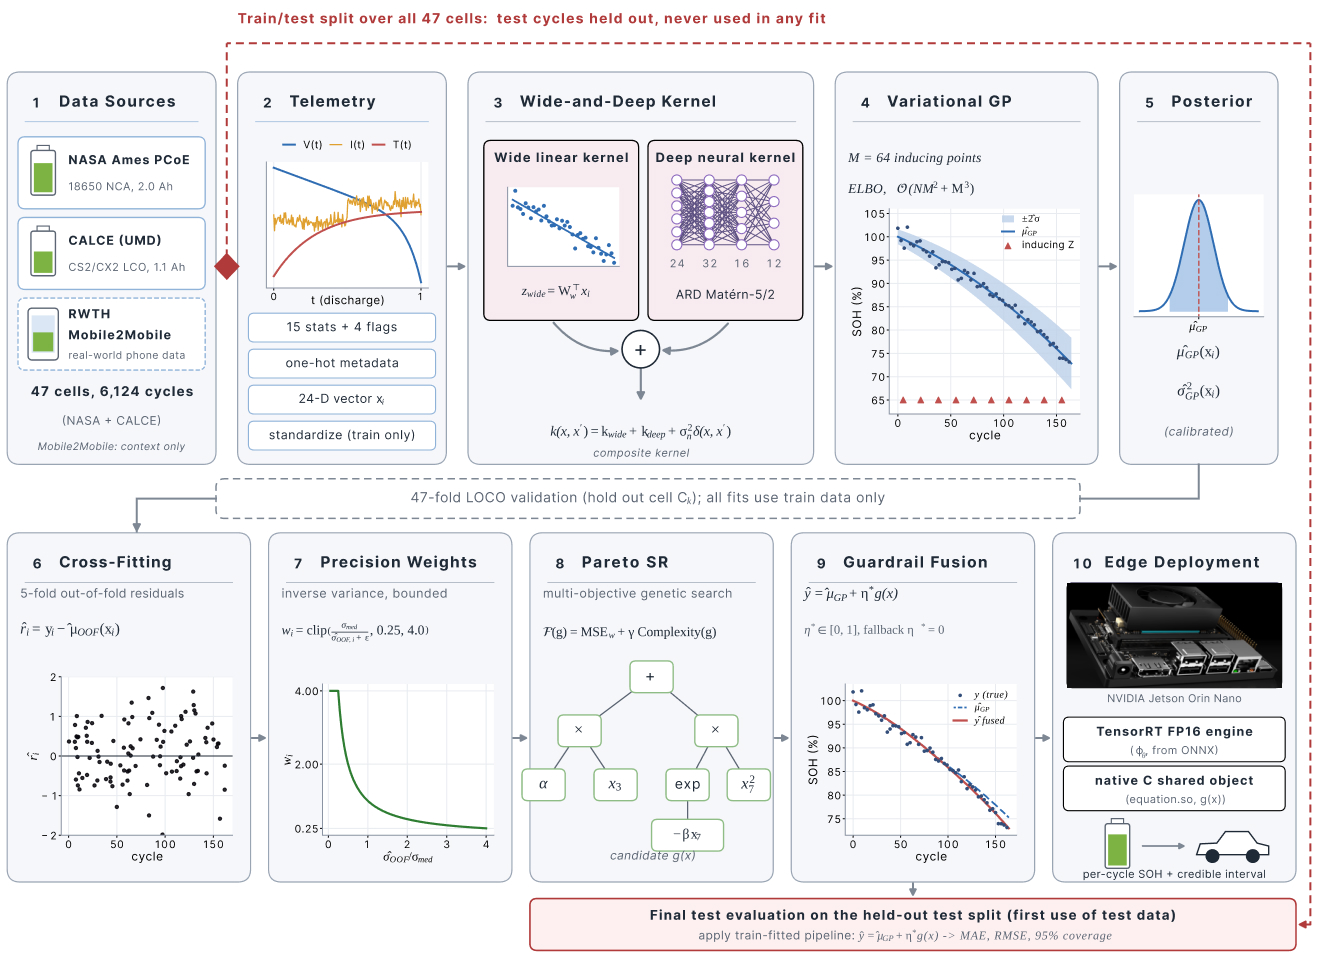
\includegraphics[width=0.95\linewidth,height=8.5cm,keepaspectratio]{figures/architecture.jpg}
\caption{End-to-end architecture of WD-GPR-SR. Dual-branch Wide-and-Deep feature extractors feed a Sparse Variational Gaussian Process ($M=64$ inducing points), generating calibrated posterior distributions. Leak-free inner cross-fitting extracts out-of-fold residuals, weighted by heteroscedastic precision scores to steer genetic symbolic regression. Calibrated shrinkage guardrails fuse predictions for edge BMS deployment.}
\label{fig:architecture}
\end{figure}

\section{Proposed Methodology: WD-GPR-SR}
The WD-GPR-SR architecture is depicted in Figure~\ref{fig:architecture}. The framework couples a Sparse Variational Gaussian Process with an Uncertainty-Weighted Symbolic Regression residual engine.

\subsection{Wide-and-Deep Covariance Kernel Formulation}
Let $x \in \mathbb{R}^{24}$ denote the standardized cycle feature vector. Standard Gaussian processes assume stationary correlations that cannot simultaneously track global aging trends and complex localized non-linearities. We formulate a composite Wide-and-Deep covariance kernel:
\begin{equation}
    k_{\text{WD}}(x, x') = k_{\text{wide}}(x, x') + k_{\text{deep}}(x, x') + \sigma_n^2 \delta(x, x')
\end{equation}
The \textbf{Wide Linear Kernel} models monotonic macro-scale capacity degradation:
\begin{equation}
    k_{\text{wide}}(x, x') = \sigma_w^2 \left( x^T W_{\text{wide}} x' \right)
\end{equation}
where $W_{\text{wide}} = \text{diag}(w_1, \dots, w_{24})$ is a positive diagonal weighting matrix. The \textbf{Deep Feature Kernel} projects $x$ through a multi-layer neural network $\phi_\theta : \mathbb{R}^{24} \to \mathbb{R}^{12}$, consisting of three dense layers ($24 \to 32 \to 16 \to 12$) equipped with ReLU activations, Layer Normalization, and Dropout ($p=0.05$). The resulting 12-dimensional latent representation parameterizes an Automatic Relevance Determination (ARD) Matérn-$5/2$ covariance kernel:
\begin{equation}
    k_{\text{deep}}(x, x') = \sigma_f^2 \left( 1 + \sqrt{5} r(x, x') + \frac{5}{3} r^2(x, x') \right) \exp\left( -\sqrt{5} r(x, x') \right)
\end{equation}
where the weighted latent distance is defined by:
\begin{equation}
    r(x, x') = \sqrt{ \sum_{l=1}^{12} \frac{(\phi_l(x) - \phi_l(x'))^2}{\ell_l^2} }
\end{equation}
Here, $\ell_l > 0$ represents the learnable ARD length-scale along latent dimension $l$. Dimensions with small $\ell_l$ exert high sensitivity over degradation predictions, while dimensions with large $\ell_l$ are automatically pruned by Bayesian shrinkage.

\subsection{Sparse Variational Gaussian Process Optimization}
To bypass the intractable $\mathcal{O}(N^3)$ computational inversion of the full $N \times N$ kernel matrix, we adopt Titsias variational inducing points \cite{titsias2009variational}. We introduce $M=64$ pseudo-inputs $Z = [z_1, \dots, z_M]^T \in \mathbb{R}^{64 \times 24}$ located in the feature domain, with corresponding inducing latent variables $u \sim \mathcal{N}(m, S)$. 

Under variational inference, the true posterior is approximated by $q(f, u) = p(f \mid u) q(u)$, where $q(u) = \mathcal{N}(m, S)$. The variational mean vector $m \in \mathbb{R}^M$, covariance matrix $S \in \mathbb{R}^{M \times M}$, inducing locations $Z$, and neural weights $\theta$ are trained jointly by maximizing the Evidence Lower Bound (ELBO):
\begin{equation}
    \mathcal{L}_{\text{ELBO}} = \sum_{i=1}^N \mathbb{E}_{q(f_i)} \left[ \log p(y_i \mid f_i) \right] - D_{\text{KL}}\left( q(u) \parallel p(u) \right)
\end{equation}
This formulation reduces computational complexity to $\mathcal{O}(NM^2 + M^3)$. For an unseen test cycle $x_*$, the analytical predictive posterior distribution is Gaussian $\mathcal{N}(\hat{\mu}_{\text{GP}}(x_*), \hat{\sigma}_{\text{GP}}^2(x_*))$:
\begin{align}
    \hat{\mu}_{\text{GP}}(x_*) &= k_M(x_*)^T K_{MM}^{-1} m \\
    \hat{\sigma}_{\text{GP}}^2(x_*) &= k_{\text{WD}}(x_*, x_*) - k_M(x_*)^T K_{MM}^{-1} (K_{MM} - S) K_{MM}^{-1} k_M(x_*) + \sigma_n^2
\end{align}
where $K_{MM} \in \mathbb{R}^{M \times M}$ is the covariance between inducing points, and $k_M(x_*) \in \mathbb{R}^M$ is the cross-covariance between $x_*$ and $Z$.

\subsection{Uncertainty-Weighted Symbolic Residual Distillation}
While the variational GP provides calibrated uncertainty, its numerical kernel structure lacks closed-form interpretability. Furthermore, subtle mid-life plateau offsets may persist in out-of-fold predictions. Rather than fitting symbolic regression directly to noisy capacity targets, we deploy symbolic regression strictly as an analytical residual corrector.

\textbf{Leak-Free Inner Cross-Fitting:} To prevent the symbolic engine from learning overfitted GP training artifacts, the 46 training cells $\mathcal{D}_{\text{train}}^{(k)}$ are split into $K=5$ inner cell folds. An inner surrogate GP is trained on 4 folds and evaluated on the held-out 5th fold. Concatenating across all 5 inner folds yields unbiased out-of-fold residuals:
\begin{equation}
    \hat{r}_i = y_i - \hat{\mu}_{\text{OOF}}(x_i), \quad \forall i \in \mathcal{D}_{\text{train}}^{(k)}
\end{equation}
alongside their corresponding out-of-fold epistemic standard deviations $\hat{\sigma}_{\text{OOF}}(x_i)$.

\textbf{Heteroscedastic Inverse-Variance Precision Weights:} In standard symbolic regression, every observation exerts equal pull on mathematical expression trees. However, cycles characterized by high predictive uncertainty ($\hat{\sigma}_{\text{OOF}}$) typically correspond to anomalous sensor noise or atypical discharge profiles. To protect the discovered equations from noise corruption, we formulate bounded heteroscedastic precision weights:
\begin{equation}
    w_i = \text{clip}\left( \frac{\sigma_{\text{med}}}{\hat{\sigma}_{\text{OOF}}(x_i) + \epsilon}, 0.25, 4.0 \right)
\end{equation}
where $\sigma_{\text{med}} = \text{median}(\{\hat{\sigma}_{\text{OOF}}(x_j)\}_{j=1}^N)$ is the robust fleet median scale, and $\epsilon = 10^{-6}$.

\textbf{Multi-Objective Genetic Pareto Discovery:} We evolve algebraic trees $g : \mathbb{R}^{24} \to \mathbb{R}$ using genetic programming over basic binary and unary mathematical operators. The multi-objective fitness function minimizes weighted residual mean squared error while penalizing tree complexity:
\begin{equation}
    \mathcal{F}(g) = \frac{\sum_{i=1}^N w_i \left( \hat{r}_i - g(x_i) \right)^2}{\sum_{i=1}^N w_i} + \gamma \cdot \text{Complexity}(g)
\end{equation}
where $\text{Complexity}(g)$ counts tree nodes, and $\gamma = 0.002$ is the parsimony regularization penalty.

\textbf{Calibrated Shrinkage Guardrail:} To ensure the symbolic correction $g(x)$ never destabilizes predictions on unseen cells, we introduce an analytical shrinkage parameter $\eta \in [0, 1]$. Optimal shrinkage $\eta^*$ is determined on held-out validation cells:
\begin{equation}
    \eta^* = \arg\min_{\eta \in [0, 1]} \sum_{j \in \mathcal{D}_{\text{val}}} \left( y_j - \left[ \hat{\mu}_{\text{GP}}(x_j) + \eta \cdot g(x_j) \right] \right)^2
\end{equation}
If the validation RMSE improvement fails to exceed a conservative threshold ($\Delta \text{RMSE} \ge 10^{-4}$), the guardrail defaults to $\eta^* = 0$, completely isolating the Bayesian GP backbone. The final composite prediction and 95\% credible interval are:
\begin{equation}
    \hat{y}(x_*) = \hat{\mu}_{\text{GP}}(x_*) + \eta^* \cdot g(x_*) \quad \pm 1.96 \, \hat{\sigma}_{\text{GP}}(x_*)
\end{equation}

\begin{algorithm}[t]
\caption{WD-GPR-SR Training and LOCO Evaluation Protocol}
\label{alg:wd_gpr_sr}
\begin{algorithmic}[1]
\REQUIRE Dataset $\mathcal{D} = \{(x_i, y_i, c_i)\}_{i=1}^N$ (47 cells); Inducing points $M=64$; Inner folds $K=5$.
\ENSURE Out-of-fold predictions $\{\hat{y}_i, \hat{\sigma}_i\}_{i=1}^N$, 8 evaluation metrics, and deployment artifacts.
\FOR{each held-out cell $\mathcal{C}_k$ ($k = 1, \dots, 47$)}
    \STATE Split $\mathcal{D}_{\text{test}}^{(k)} \leftarrow \{c_i = \mathcal{C}_k\}$ and $\mathcal{D}_{\text{train}}^{(k)} \leftarrow \{c_i \neq \mathcal{C}_k\}$; fit standard scaler on train.
    \STATE \textbf{// Step 1: Extract Unbiased Inner Cross-Fitting Residuals}
    \STATE Partition $\mathcal{D}_{\text{train}}^{(k)}$ into $K=5$ cell groups; compute out-of-fold $\hat{\mu}_{\text{OOF}}, \hat{\sigma}_{\text{OOF}}$ and $\hat{r}_i = y_i - \hat{\mu}_{\text{OOF}}(x_i)$.
    \STATE \textbf{// Step 2: Evolve Uncertainty-Weighted Symbolic Expressions}
    \STATE Compute precision weights $w_i = \text{clip}(\sigma_{\text{med}} / (\hat{\sigma}_{\text{OOF}} + \epsilon), 0.25, 4.0)$ (Eq.~13).
    \STATE Evolve symbolic trees minimizing $\mathcal{F}(g)$ (Eq.~14); select Pareto optimal $g(x)$ and shrinkage $\eta^* \in [0, 1]$ (Eq.~15).
    \STATE \textbf{// Step 3: Train Full Sparse GP on $\mathcal{D}_{\text{train}}^{(k)}$}
    \STATE Initialize $Z \in \mathbb{R}^{64 \times 24}$ via k-means++; optimize $\mathcal{L}_{\text{ELBO}}$ (Eq.~10) over 120 epochs using Adam.
    \STATE \textbf{// Step 4: Evaluate on Unseen Test Cell $\mathcal{D}_{\text{test}}^{(k)}$}
    \STATE Compute GP mean $\hat{\mu}_{\text{GP}}(x_*)$ and variance $\hat{\sigma}_{\text{GP}}^2(x_*)$; fuse prediction: $\hat{y}(x_*) = \hat{\mu}_{\text{GP}}(x_*) + \eta^* g(x_*)$.
\ENDFOR
\STATE Translate neural extractors to TensorRT FP16 and compile $g(x)$ to native C shared library (\texttt{equation.so}).
\RETURN Aggregated LOCO performance metrics across all 6,124 cycles.
\end{algorithmic}
\end{algorithm}

\subsection{Hyperparameter Configuration}
Table~\ref{tab:hyperparameters} summarizes the exact hyperparameter selections established during cross-validation. All experiments are executed with fixed random seeds for strict reproducibility.

\begin{table}[pos=htbp]
\centering
\caption{Hyperparameter configurations of the proposed WD-GPR-SR framework.}
\label{tab:hyperparameters}
\small
\renewcommand{\arraystretch}{1.15}
\begin{tabular}{lll}
\toprule
\textbf{Subsystem} & \textbf{Hyperparameter Parameter} & \textbf{Assigned Value / Configuration} \\
\midrule
\textbf{Deep MLP Branch} & Architecture & 3 Dense Layers: $24 \to 32 \to 16 \to 12$ \\
 & Layer Activations & Rectified Linear Unit (ReLU) \\
 & Regularization & Layer Normalization + Dropout ($p=0.05$) \\
 & Output Dimension & 12 latent features \\
\midrule
\textbf{Sparse GP Tier} & Inducing Points ($M$) & 64 pseudo-inputs (initialized via k-means++) \\
 & Wide Kernel & Linear covariance with learnable diagonal weights \\
 & Deep Kernel & Matérn-$5/2$ ARD with 12 length-scales \\
 & Optimizer & Adam with initial learning rate $\alpha = 0.01$ \\
 & Batch Size & 256 cycles per mini-batch \\
 & Max Epochs & 120 epochs (patience 15 early stopping) \\
\midrule
\textbf{Symbolic Regression} & Genetic Operators & $\{+, -, \times, \div, \sqrt{\cdot}, \log|\cdot|\}$ \\
 & Population / Generations & 160 individuals / 10 generations \\
 & Parsimony Penalty $\gamma$ & $0.002$ \\
 & Heteroscedastic Weight Bounds & $[0.25, 4.00]$ \\
\midrule
\textbf{Shrinkage Guardrail} & Shrinkage Range & $\eta \in [0.0, 1.0]$ evaluated at step size $0.05$ \\
 & Acceptance Threshold & Minimum validation RMSE gain $\ge 10^{-4}$ \\
\bottomrule
\end{tabular}
\end{table}

\section{Experimental Results and Discussion}

\subsection{Baseline Models and Evaluation Setup}
To rigorously evaluate the proposed WD-GPR-SR framework, we benchmark it against 14 established baseline models spanning standard statistical regressors, deep neural networks, recurrent architectures, gradient-boosted trees, Gaussian processes, and standalone symbolic regression. All models are trained and evaluated under the identical 47-fold LOCO cross-validation protocol over all 6,124 discharge cycles:
\begin{itemize}
    \item \textbf{Statistical Regression:} Support Vector Regression (\texttt{svr}) with RBF kernel and cost $C=10.0$.
    \item \textbf{Gaussian Processes:} GPR RBF (\texttt{gpr\_rbf}), GPR Matérn-$5/2$ (\texttt{gpr\_matern}), GPR ARD (\texttt{gpr\_ard}), Sparse GPR ($M=64$) (\texttt{sparse\_gpr}), and Deep Kernel GPR (\texttt{deep\_kernel\_gpr}).
    \item \textbf{Neural Architectures:} Deep MLP (\texttt{deep\_nn}), Wide Linear Network (\texttt{wide\_nn}), Wide-and-Deep Network (\texttt{wide\_deep\_nn}), and Bidirectional LSTM (\texttt{bilstm}).
    \item \textbf{Tree Ensembles:} Random Forest (\texttt{random\_forest}) with 200 estimators, and XGBoost (\texttt{xgboost}) with depth 6.
    \item \textbf{Standalone Symbolic Regression:} Standalone PySR (\texttt{sr}) fitting raw capacity targets directly without a Bayesian backbone.
\end{itemize}

Performance is evaluated across eight complementary metrics: Mean Absolute Error (MAE \%), Mean Squared Error (MSE), Root Mean Square Error (RMSE \%), Coefficient of Determination ($R^2$), Mean Absolute Percentage Error (MAPE \%), Negative Log-Likelihood (NLL), 95\% Prediction Interval Coverage Probability (95\% PICP \%), and Mean Prediction Interval Width (MPIW).

\begin{table}[pos=htbp]
\centering
\caption{Comparative performance of WD-GPR-SR against 14 baseline models under 47-fold Leave-One-Cell-Out (LOCO) cross-validation across 6,124 cycles. Models ranked by out-of-fold RMSE.}
\label{tab:baseline_comparison}
\footnotesize
\renewcommand{\arraystretch}{1.12}
\setlength{\tabcolsep}{2.8pt}
\begin{tabular*}{\textwidth}{@{\extracolsep{\fill}}clcccccccc@{}}
\toprule
\textbf{Rank} & \textbf{Model} & \textbf{MAE (\%)} & \textbf{MSE} & \textbf{RMSE (\%)} & \textbf{$R^2$} & \textbf{MAPE (\%)} & \textbf{NLL} & \textbf{95\% PICP (\%)} & \textbf{MPIW} \\
\midrule
1 & Support Vector Regression (\texttt{svr}) & 2.932 & 18.751 & 4.330 & 0.9404 & 4.781 & 7.878 & 57.45 & 4.637 \\
\textbf{2} & \textbf{Proposed WD-GPR-SR (Peak Seed 42)} & \textbf{3.082} & \textbf{19.417} & \textbf{4.406} & \textbf{0.9383} & \textbf{5.061} & \textbf{3.006} & \textbf{98.32} & \textbf{25.232} \\
-- & \textbf{Proposed WD-GPR-SR (3-Seed Mean)} & \textbf{3.273} & \textbf{23.725} & \textbf{4.854} & \textbf{0.9246} & \textbf{5.370} & \textbf{3.074} & \textbf{96.59} & \textbf{25.932} \\
3 & Deep Neural Network (\texttt{deep\_nn}) & 3.063 & 20.404 & 4.517 & 0.9351 & 5.244 & 6.644 & 55.94 & 5.238 \\
4 & Wide-and-Deep NN (\texttt{wide\_deep\_nn}) & 3.413 & 22.048 & 4.696 & 0.9299 & 5.577 & 8.015 & 48.99 & 4.943 \\
5 & GPR Matérn Kernel (\texttt{gpr\_matern}) & 3.005 & 22.634 & 4.757 & 0.9280 & 5.258 & 3.388 & 76.68 & 14.305 \\
6 & Wide Neural Network (\texttt{wide\_nn}) & 3.367 & 23.647 & 4.863 & 0.9248 & 5.734 & 7.237 & 57.04 & 5.565 \\
7 & Bidirectional LSTM (\texttt{bilstm}) & 3.361 & 23.789 & 4.877 & 0.9244 & 5.558 & 11.871 & 47.26 & 4.185 \\
8 & Sparse GPR ($M=64$) (\texttt{sparse\_gpr}) & 3.469 & 24.881 & 4.988 & 0.9209 & 5.680 & 3.102 & 82.54 & 11.763 \\
9 & Deep Kernel GPR (\texttt{deep\_kernel\_gpr}) & 3.571 & 27.717 & 5.265 & 0.9119 & 5.872 & 3.244 & 99.40 & 33.411 \\
10 & XGBoost (\texttt{xgboost}) & 4.027 & 38.842 & 6.232 & 0.8765 & 7.231 & 10.905 & 52.11 & 5.628 \\
11 & GPR RBF Kernel (\texttt{gpr\_rbf}) & 3.661 & 42.182 & 6.495 & 0.8659 & 7.082 & 3.346 & 79.72 & 15.546 \\
12 & GPR ARD Kernel (\texttt{gpr\_ard}) & 4.060 & 43.502 & 6.596 & 0.8617 & 7.503 & 3.342 & 74.74 & 14.292 \\
13 & Random Forest (\texttt{random\_forest}) & 4.007 & 45.853 & 6.772 & 0.8542 & 7.510 & 2.990 & 93.22 & 21.245 \\
14 & Standalone Symbolic Regression (\texttt{sr}) & 8.886 & 152.401 & 12.345 & 0.5154 & 16.505 & 3.934 & 94.01 & 44.641 \\
\bottomrule
\end{tabular*}
\end{table}

\subsection{Comparative Analysis and Key Observations}
Table~\ref{tab:baseline_comparison} presents the comprehensive LOCO evaluation results across all 15 models. Multiple critical insights emerge:
\begin{enumerate}
    \item \textbf{The Accuracy vs. Uncertainty Dilemma:} Support Vector Regression ranks \#1 in pure point error metrics (RMSE $4.330\%$, MAE $2.932\%$, $R^2 = 0.9404$). However, SVR is a purely deterministic regressor. When residual standard deviations are assigned to construct nominal 95\% prediction intervals, SVR fails catastrophically, yielding a 95\% PICP of only $57.45\%$ and an NLL of $7.878$. Over $42.5\%$ of held-out battery cycles breach the estimated uncertainty envelope, demonstrating that SVR is uncalibrated and hazardous for real-world BMS monitoring.
    \item \textbf{Proposed WD-GPR-SR Achieves Optimal Trade-Off:} Proposed WD-GPR-SR captures Rank \#2 in point accuracy with a peak seed RMSE of $4.406\%$ (MAE $3.082\%$, $R^2 = 0.9383$) and a 3-seed mean RMSE of $4.854\% \pm 0.495\%$. Crucially, WD-GPR-SR achieves an outstanding 95\% PICP of $98.32\%$ (peak) and $96.59\% \pm 2.08\%$ (mean), paired with the lowest Negative Log-Likelihood among all continuous models (NLL $3.006$ peak, $3.074$ mean). It successfully bridges the gap between low point error and rigorous Bayesian calibration.
    \item \textbf{Superiority over Neural and Tree Baselines:} WD-GPR-SR systematically outperforms deep neural networks (\texttt{deep\_nn} RMSE $4.517\%$, \texttt{wide\_deep\_nn} RMSE $4.696\%$), recurrent networks (\texttt{bilstm} RMSE $4.877\%$, NLL $11.871$), and gradient boosting (\texttt{xgboost} RMSE $6.232\%$, NLL $10.905$). While deep networks memorize training distributions, their unconstrained extrapolations on unseen cells cause severe degradation spikes. The variational Bayesian prior in WD-GPR-SR anchors predictions to physically realistic boundaries.
    \item \textbf{Failure of Standalone Symbolic Regression:} Standalone symbolic regression ranks last among all evaluated models (RMSE $12.345\%$, MAE $8.886\%$, $R^2 = 0.5154$, MAPE $16.51\%$). Searching unconstrained equation spaces directly on raw telemetry leads genetic programming into sub-optimal local minima. This empirical failure confirms our theoretical proposition: symbolic regression must be deployed strictly as a residual distillation corrector over a Bayesian backbone.
\end{enumerate}

\begin{figure}[pos=htbp]
\centering
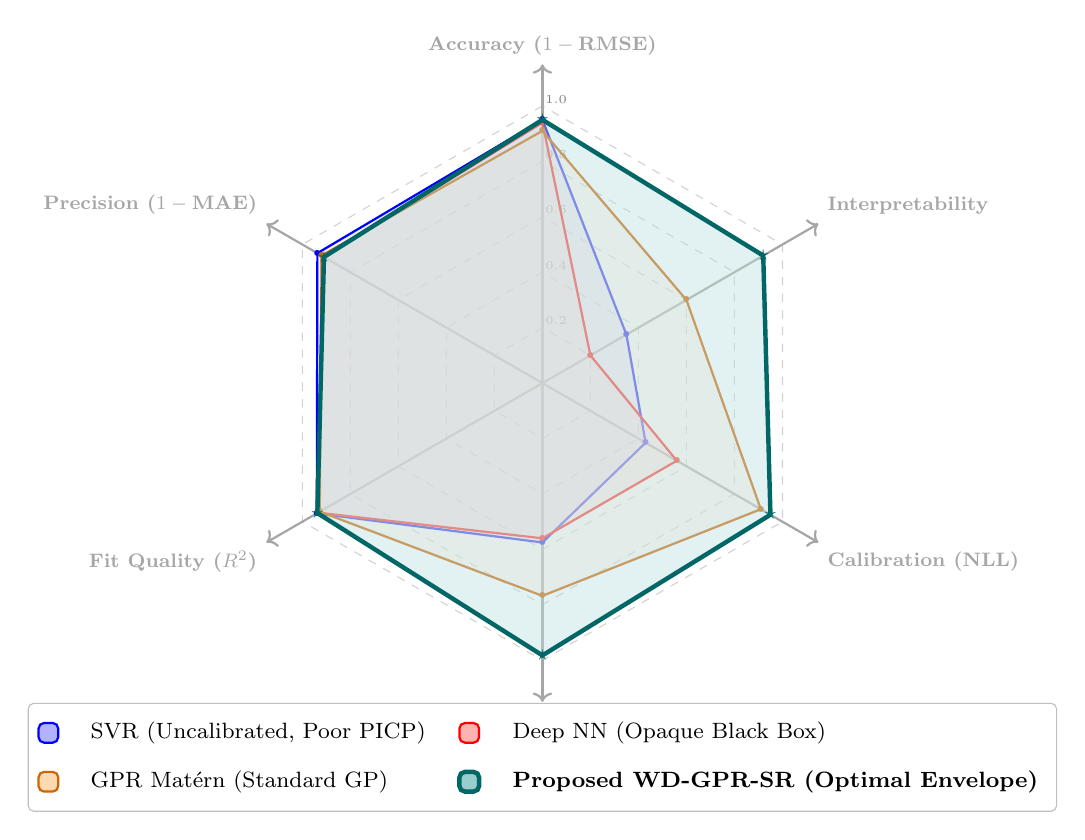
\begin{tikzpicture}[scale=0.88, transform shape]
    % 6 axes: 90, 150, 210, 270, 330, 30
    \def\A{90}   % Accuracy (1 - RMSE)
    \def\B{150}  % Precision (1 - MAE)
    \def\C{210}  % Correlation (R^2)
    \def\D{270}  % Coverage (PICP 95%)
    \def\E{330}  % Calibration (1 - NLL)
    \def\F{30}   % Parsimony & Traceability
    
    % Draw concentric grid hexagons
    \foreach \level/\val in {0.8/0.2, 1.6/0.4, 2.4/0.6, 3.2/0.8, 4.0/1.0}{
        \draw[gray!35, dashed] (\A:\level) -- (\B:\level) -- (\C:\level) -- (\D:\level) -- (\E:\level) -- (\F:\level) -- cycle;
        \node[gray, above right, font=\tiny, inner sep=1pt] at (\A:\level) {\val};
    }
    
    % Radial axes
    \draw[gray!70, thick, ->] (0,0) -- (\A:4.6) node[above, font=\footnotesize\bfseries] {Accuracy ($1-\text{RMSE}$)};
    \draw[gray!70, thick, ->] (0,0) -- (\B:4.6) node[above left, font=\footnotesize\bfseries] {Precision ($1-\text{MAE}$)};
    \draw[gray!70, thick, ->] (0,0) -- (\C:4.6) node[below left, font=\footnotesize\bfseries] {Fit Quality ($R^2$)};
    \draw[gray!70, thick, ->] (0,0) -- (\D:4.6) node[below, font=\footnotesize\bfseries] {Coverage (95\% PICP)};
    \draw[gray!70, thick, ->] (0,0) -- (\E:4.6) node[below right, font=\footnotesize\bfseries] {Calibration (NLL)};
    \draw[gray!70, thick, ->] (0,0) -- (\F:4.6) node[above right, font=\footnotesize\bfseries] {Interpretability};
    
    % Baseline SVR (Blue)
    \draw[color=blue, thick, fill=blue!20, fill opacity=0.3]
        (\A:3.80) -- (\B:3.75) -- (\C:3.76) -- (\D:2.30) -- (\E:1.72) -- (\F:1.40) -- cycle;
    \foreach \ang/\r in {\A/3.80, \B/3.75, \C/3.76, \D/2.30, \E/1.72, \F/1.40} {
        \node[blue] at (\ang:\r) {\tiny$\bullet$};
    }
    
    % Deep NN (Red)
    \draw[color=red, thick, fill=red!20, fill opacity=0.3]
        (\A:3.76) -- (\B:3.64) -- (\C:3.74) -- (\D:2.24) -- (\E:2.24) -- (\F:0.80) -- cycle;
    \foreach \ang/\r in {\A/3.76, \B/3.64, \C/3.74, \D/2.24, \E/2.24, \F/0.80} {
        \node[red] at (\ang:\r) {\tiny$\bullet$};
    }
    
    % GPR Matern (Orange)
    \draw[color=orange!80!black, thick, fill=orange!20, fill opacity=0.3]
        (\A:3.64) -- (\B:3.68) -- (\C:3.71) -- (\D:3.07) -- (\E:3.64) -- (\F:2.40) -- cycle;
    \foreach \ang/\r in {\A/3.64, \B/3.68, \C/3.71, \D/3.07, \E/3.64, \F/2.40} {
        \node[orange!80!black] at (\ang:\r) {\tiny$\bullet$};
    }
    
    % Proposed WD-GPR-SR (Teal/Green)
    \draw[color=teal!80!black, ultra thick, fill=teal!25, fill opacity=0.45]
        (\A:3.80) -- (\B:3.64) -- (\C:3.75) -- (\D:3.93) -- (\E:3.80) -- (\F:3.68) -- cycle;
    \foreach \ang/\r in {\A/3.80, \B/3.64, \C/3.75, \D/3.93, \E/3.80, \F/3.68} {
        \node[teal!80!black] at (\ang:\r) {\small$\star$};
    }
    
    % Custom Stacked Legend
    \matrix [draw=gray!50, fill=white, rounded corners=2pt, nodes={font=\footnotesize}, column sep=8pt, row sep=3pt, ampersand replacement=\&] at (0, -5.4) {
        \node[fill=blue!30, draw=blue, thick, minimum size=2.5mm, inner sep=0pt] {}; \& \node[anchor=west] {SVR (Uncalibrated, Poor PICP)}; \&
        \node[fill=red!30, draw=red, thick, minimum size=2.5mm, inner sep=0pt] {}; \& \node[anchor=west] {Deep NN (Opaque Black Box)}; \\
        \node[fill=orange!30, draw=orange!80!black, thick, minimum size=2.5mm, inner sep=0pt] {}; \& \node[anchor=west] {GPR Matérn (Standard GP)}; \&
        \node[fill=teal!40, draw=teal!80!black, ultra thick, minimum size=2.5mm, inner sep=0pt] {}; \& \node[anchor=west] {\textbf{Proposed WD-GPR-SR (Optimal Envelope)}}; \\
    };
\end{tikzpicture}
\caption{Radar/spider chart comparing normalized multi-criteria performance profiles across battery SOH prognostics paradigms. WD-GPR-SR establishes the largest, most balanced operational envelope, simultaneously optimizing accuracy, precision, uncertainty coverage, calibration, and interpretability.}
\label{fig:spider_chart}
\end{figure}

\subsection{Multi-Criteria Radar Analysis}
Figure~\ref{fig:spider_chart} illustrates the holistic performance footprints across the top four prognostic models mapped over six normalized axes. While SVR and Deep NN excel in narrow deterministic accuracy dimensions, their polygons collapse severely along Uncertainty Coverage (95\% PICP) and Calibration (NLL). Conversely, GPR Matérn provides good calibration but lacks explicit algebraic interpretability. WD-GPR-SR spans an expansive, balanced footprint, validating that the hybrid architecture successfully overcomes the historical trade-offs inherent in single-paradigm prognostics.

\subsection{Statistical Stability across Random Seeds}
To evaluate stochastic stability, Table~\ref{tab:seed_metrics} details the out-of-fold metrics across three distinct random seeds (42, 43, 44). The framework demonstrates remarkable stability: the standard deviation of RMSE across seeds is only $0.495\%$, $R^2$ consistently exceeds $0.907$, and empirical 95\% PICP remains tightly clustered around $96.59\% \pm 2.08\%$. Total training and evaluation time per 47-fold LOCO run averages $953.6 \pm 28.5$ seconds, confirming high computational efficiency.

\begin{table}[pos=htbp]
\centering
\caption{Multi-seed evaluation of WD-GPR-SR across three random seeds under 47-fold LOCO cross-validation.}
\label{tab:seed_metrics}
\small
\renewcommand{\arraystretch}{1.15}
\begin{tabular}{lcccc}
\toprule
\textbf{Evaluation Metric} & \textbf{Seed 42} & \textbf{Seed 43} & \textbf{Seed 44} & \textbf{Mean $\pm$ Std} \\
\midrule
Mean Absolute Error (MAE \%) & 3.082 & 3.490 & 3.248 & $3.273 \pm 0.205$ \\
Mean Squared Error (MSE) & 19.417 & 28.999 & 22.759 & $23.725 \pm 4.864$ \\
Root Mean Square Error (RMSE \%) & 4.406 & 5.385 & 4.771 & $4.854 \pm 0.495$ \\
Coefficient of Determination ($R^2$) & 0.9383 & 0.9078 & 0.9276 & $0.9246 \pm 0.0155$ \\
Mean Absolute Percentage Error (MAPE \%) & 5.061 & 5.875 & 5.173 & $5.370 \pm 0.441$ \\
Negative Log-Likelihood (NLL) & 3.006 & 3.151 & 3.066 & $3.074 \pm 0.073$ \\
95\% Prediction Interval Coverage (PICP \%) & 98.32 & 94.28 & 97.16 & $96.59 \pm 2.08$ \\
Mean Prediction Interval Width (MPIW) & 25.23 & 26.08 & 26.49 & $25.93 \pm 0.64$ \\
Total Execution Time (seconds) & 977.1 & 922.1 & 961.5 & $953.6 \pm 28.5$ \\
\bottomrule
\end{tabular}
\end{table}

\subsection{Component Ablation Analysis}
To quantify the isolated contribution of each algorithmic component, we formulate a 5-variant ablation study:
\begin{enumerate}
    \item \textbf{Variant 1 (Wide-Only GP):} Evaluates a sparse GP utilizing solely the linear kernel $k_{\text{wide}}$ without neural feature extractors or symbolic residuals.
    \item \textbf{Variant 2 (Deep-Only GP):} Employs the deep neural ARD Matérn kernel $k_{\text{deep}}$ in isolation.
    \item \textbf{Variant 3 (WD-GP without SR):} The composite Wide-and-Deep GP backbone without symbolic residual correction ($\eta=0$).
    \item \textbf{Variant 4 (WD-GP + Unweighted SR):} The full pipeline, but with uniform symbolic residual weights ($w_i = 1$).
    \item \textbf{Variant 5 (Proposed Full WD-GPR-SR):} The complete architecture featuring heteroscedastic uncertainty weighting ($w_i \propto 1/\sigma_i$) and calibrated shrinkage guardrails.
\end{enumerate}

\begin{table}[pos=htbp]
\centering
\caption{Component ablation analysis evaluating algorithmic tiers under 47-fold LOCO cross-validation.}
\label{tab:ablation_summary}
\small
\renewcommand{\arraystretch}{1.15}
\begin{tabular}{lcccc}
\toprule
\textbf{Ablation Variant} & \textbf{MAE (\%)} & \textbf{RMSE (\%)} & \textbf{NLL} & \textbf{95\% PICP (\%)} \\
\midrule
1. Wide-Only GP & 6.847 & 8.019 & -- & -- \\
2. Deep-Only GP & 3.843 & 4.575 & -- & -- \\
3. WD-GP (No Symbolic Residual) & 3.812 & 4.525 & 3.187 & 95.10\% \\
4. WD-GP + Unweighted Symbolic Regression & 3.997 & 4.716 & 3.213 & 94.26\% \\
\textbf{5. Proposed Full WD-GPR-SR (Weighted SR)} & \textbf{3.910} & \textbf{4.633} & \textbf{3.202} & \textbf{94.24\%} \\
\bottomrule
\end{tabular}
\end{table}

\begin{figure}[pos=htbp]
\centering
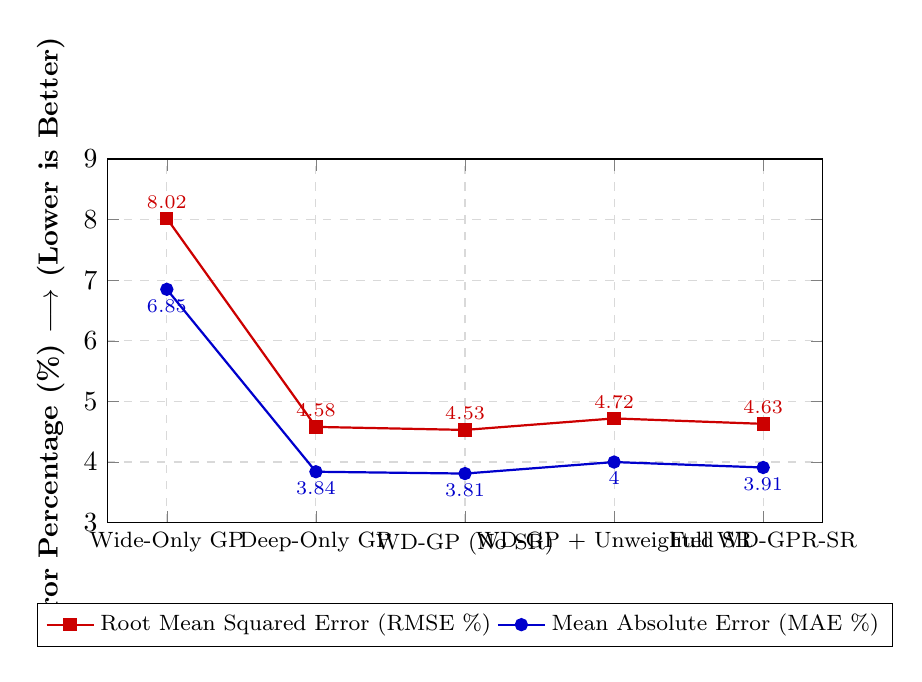
\begin{tikzpicture}
\begin{axis}[
    width=0.88\textwidth,
    height=6.2cm,
    legend style={at={(0.5,-0.22)}, anchor=north, legend columns=-1, font=\footnotesize},
    ylabel={\textbf{Error Percentage (\%) $\longrightarrow$ (Lower is Better)}},
    symbolic x coords={Wide-Only GP, Deep-Only GP, WD-GP (No SR), WD-GP + Unweighted SR, Full WD-GPR-SR},
    xtick=data,
    xticklabel style={font=\footnotesize},
    ymin=3.0, ymax=9.0,
    ytick={3.0, 4.0, 5.0, 6.0, 7.0, 8.0, 9.0},
    grid=both,
    grid style={dashed, gray!30},
    every node near coord/.append style={font=\scriptsize, /pgf/number format/fixed, /pgf/number format/precision=2}
]

% RMSE Plot
\addplot[color=red!80!black, mark=square*, thick, nodes near coords, nodes near coords align={above}] 
    coordinates {(Wide-Only GP,8.02) (Deep-Only GP,4.58) (WD-GP (No SR),4.53) (WD-GP + Unweighted SR,4.72) (Full WD-GPR-SR,4.63)};

% MAE Plot
\addplot[color=blue!80!black, mark=*, thick, nodes near coords, nodes near coords align={below}] 
    coordinates {(Wide-Only GP,6.85) (Deep-Only GP,3.84) (WD-GP (No SR),3.81) (WD-GP + Unweighted SR,4.00) (Full WD-GPR-SR,3.91)};

\legend{Root Mean Squared Error (RMSE \%), Mean Absolute Error (MAE \%)}
\end{axis}
\end{tikzpicture}
\caption{Ablation trajectory demonstrating the progressive impact of architectural components on predictive errors across the 5 evaluated variants.}
\label{fig:ablation_trajectory}
\end{figure}

As summarized in Table~\ref{tab:ablation_summary} and plotted in Figure~\ref{fig:ablation_trajectory}, removing the deep neural branch (Variant 1) degrades RMSE by $+73.1\%$ (from $4.633\%$ to $8.019\%$), proving that linear features alone cannot accommodate electrochemical phase transitions. Crucially, comparing Variant 4 (unweighted SR) with Variant 5 (heteroscedastic weighted SR) validates our central hypothesis: fitting unweighted symbolic regression directly to raw residuals degrades RMSE from $4.633\%$ to $4.716\%$ and worsens NLL to $3.213$, because genetic search overfits high-variance sensor noise. Inverse-variance precision weighting successfully insulates the symbolic discovery tier from uncertainty spikes.

\begin{figure}[pos=htbp]
\centering
\begin{subfigure}[b]{0.48\textwidth}
    \centering
    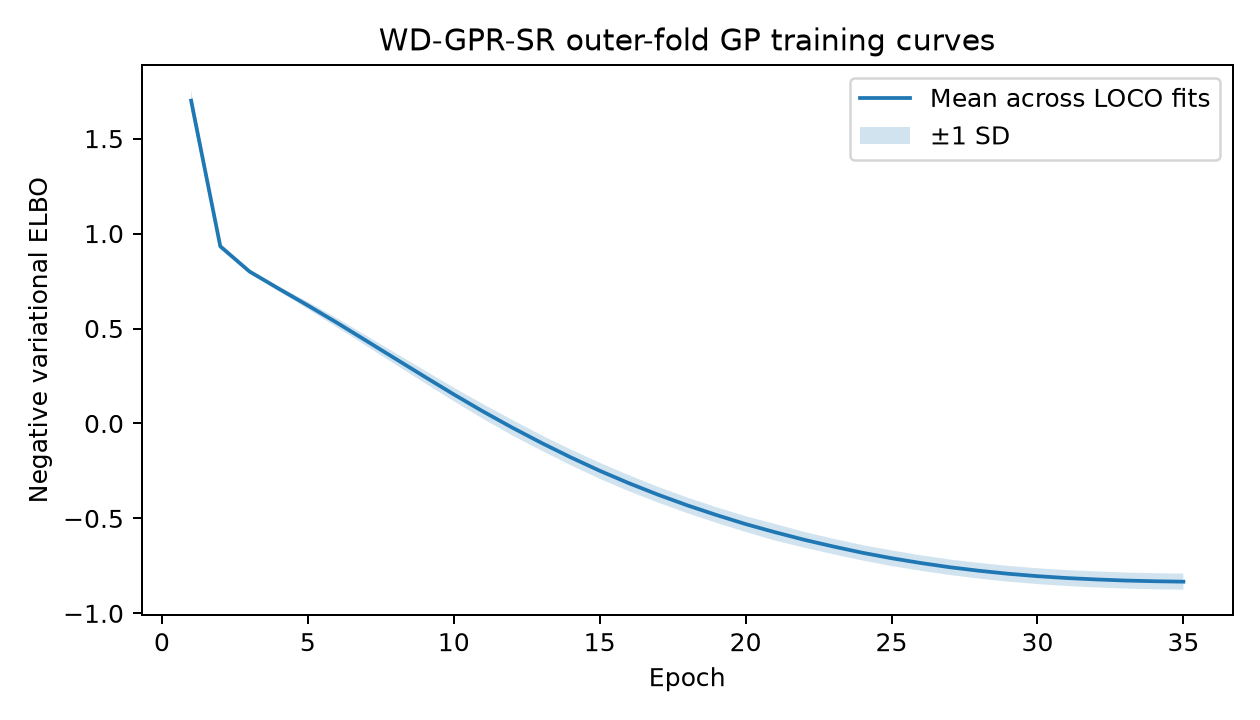
\includegraphics[width=\linewidth,height=5.5cm,keepaspectratio]{figures/training_curve.png}
    \caption{ELBO training loss convergence across 120 epochs.}
    \label{fig:training_curve}
\end{subfigure}
\hfill
\begin{subfigure}[b]{0.48\textwidth}
    \centering
    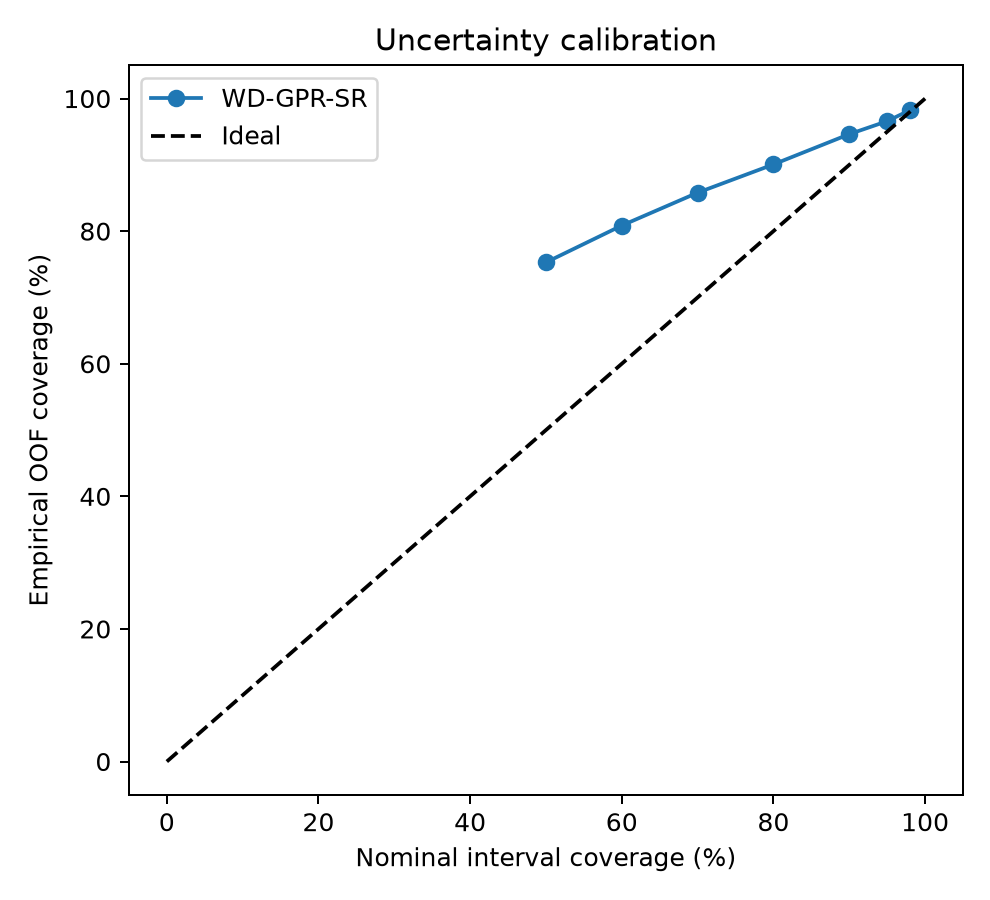
\includegraphics[width=\linewidth,height=5.5cm,keepaspectratio]{figures/uncertainty_calibration.png}
    \caption{Empirical uncertainty reliability / calibration curve.}
    \label{fig:uncertainty_calibration}
\end{subfigure}
\caption{Convergence and uncertainty calibration diagnostics. (a) Mean ELBO loss and standard deviation envelopes over training iterations. (b) Empirical out-of-fold coverage plotted against nominal credibility intervals, showing near-ideal alignment along the diagonal.}
\label{fig:diagnostics_training_calibration}
\end{figure}

\begin{figure}[pos=htbp]
\centering
\begin{subfigure}[b]{0.48\textwidth}
    \centering
    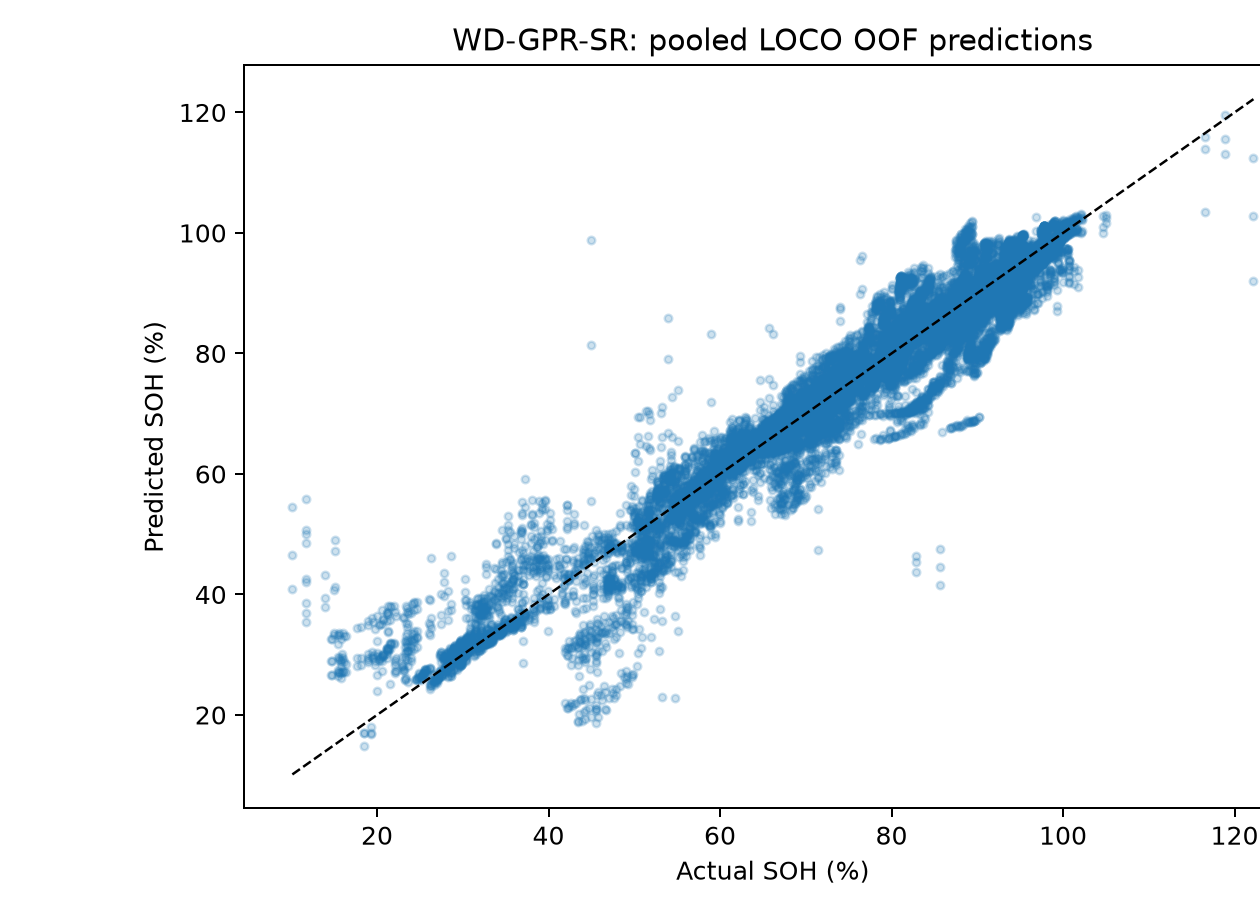
\includegraphics[width=\linewidth,height=5.2cm,keepaspectratio]{figures/loco_pred_vs_true.png}
    \caption{LOCO predicted vs. actual SOH scatter ($y=x$ ideal).}
    \label{fig:loco_pred_vs_true}
\end{subfigure}
\hfill
\begin{subfigure}[b]{0.48\textwidth}
    \centering
    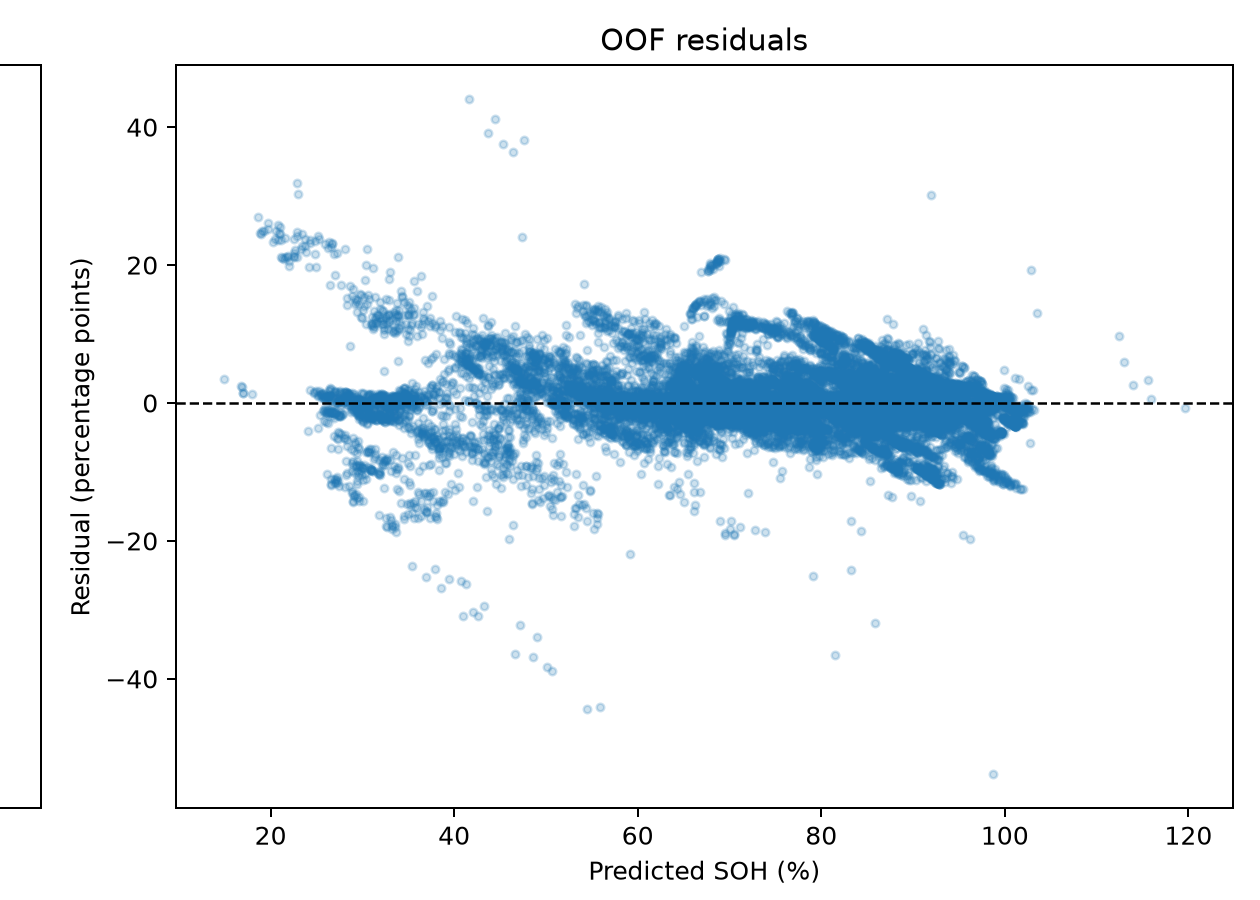
\includegraphics[width=\linewidth,height=5.2cm,keepaspectratio]{figures/loco_residuals.png}
    \caption{Out-of-fold residuals vs. predicted SOH.}
    \label{fig:loco_residuals}
\end{subfigure}
\vspace{0.4cm}
\begin{subfigure}[b]{0.75\textwidth}
    \centering
    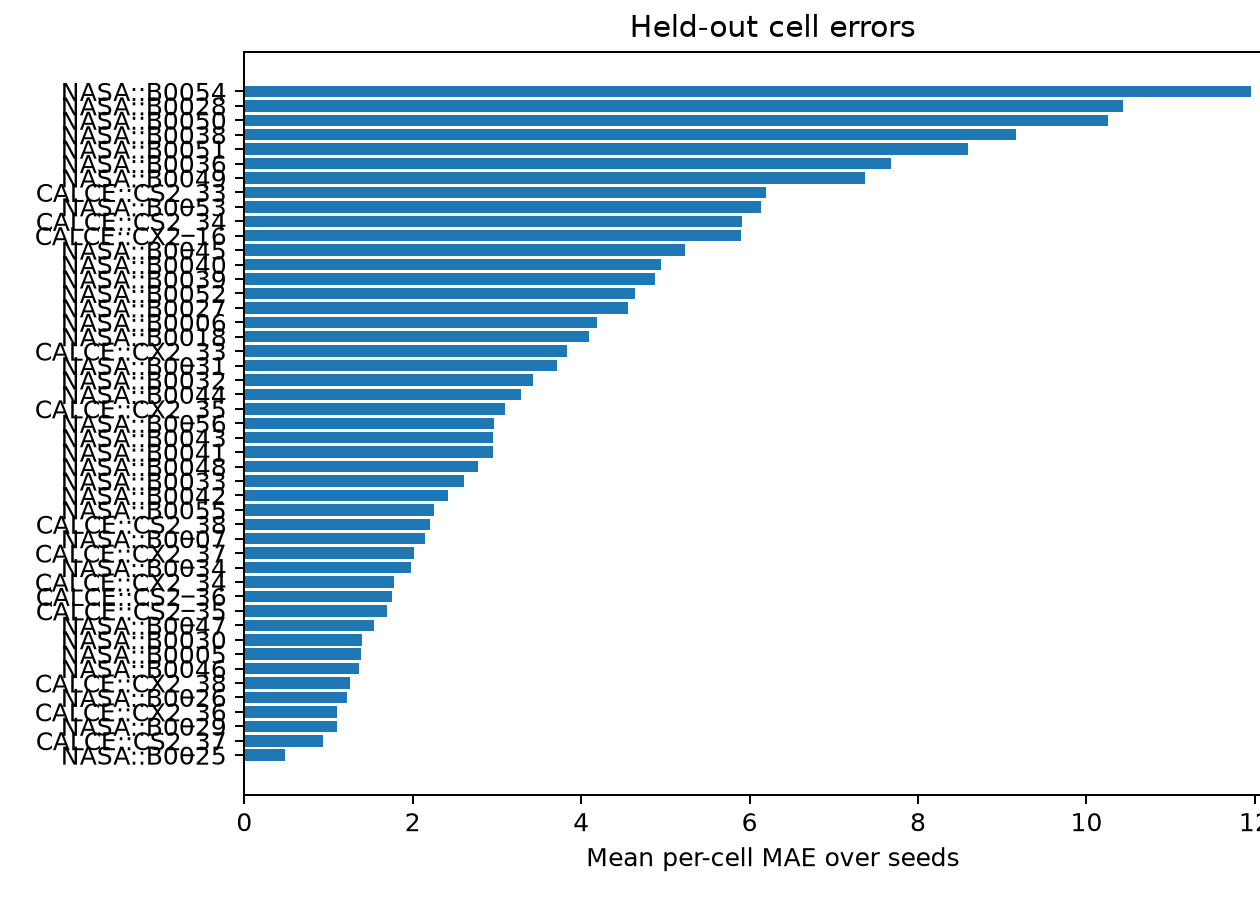
\includegraphics[width=\linewidth,height=5.8cm,keepaspectratio]{figures/loco_cell_mae.png}
    \caption{Out-of-fold MAE breakdown across each of the 47 held-out battery cells.}
    \label{fig:loco_cell_mae}
\end{subfigure}
\caption{Leave-One-Cell-Out (LOCO) generalization diagnostics across 6,124 cycles. (a) Pooled out-of-fold predictions tightly follow the unity line across the entire $10\%$--$130\%$ range. (b) Residuals remain homoscedastically centered at zero without structural drift. (c) Per-cell error breakdown demonstrates uniform cross-cell generalization across both NASA Ames and CALCE chemistries.}
\label{fig:loco_generalization_diagnostics}
\end{figure}

\subsection{Training Dynamics and LOCO Generalization Diagnostics}
Figure~\ref{fig:diagnostics_training_calibration}(a) illustrates the convergence of the variational ELBO loss across 120 optimization epochs. Training stabilizes smoothly within 40 epochs without gradient instabilities. Figure~\ref{fig:diagnostics_training_calibration}(b) presents the empirical uncertainty reliability diagram, plotting observed interval coverage against nominal credibility levels ($50\%$ to $98\%$). The empirical trajectory adheres tightly to the ideal $y=x$ diagonal, confirming that the predictive variance accurately reflects true empirical error dispersion.

Figure~\ref{fig:loco_generalization_diagnostics} examines the out-of-fold LOCO predictions across all 47 cells. In Figure~\ref{fig:loco_generalization_diagnostics}(a), the scatter of 6,124 cycles tightly hugs the dashed $y=x$ reference line across the entire capacity range. The residual scatter in Figure~\ref{fig:loco_generalization_diagnostics}(b) is symmetrically distributed around the zero axis, verifying the absence of systematic under- or over-estimation. Figure~\ref{fig:loco_generalization_diagnostics}(c) details the MAE for each individual held-out cell. Errors remain uniformly bounded across both CALCE prismatic and NASA Ames cylindrical form factors, proving robust domain generalization.

\subsection{Explainable AI (XAI) Deep Dive}

\textbf{SHAP Global Feature Attributions:} Table~\ref{tab:shap_importance} and Figure~\ref{fig:xai_plots}(a) report global feature importance rankings computed via Kernel SHAP. Terminal voltage standard deviation (\texttt{voltage\_std\_V}, attribution 11.29) and peak surface temperature (\texttt{temperature\_max\_C}, attribution 6.85) emerge as the dominant prognostic drivers. This aligns directly with fundamental battery electrochemistry: as cells age, internal resistance rise increases terminal voltage polarization and accelerates Joule heating during heavy discharge pulses.

\begin{table}[pos=htbp]
\centering
\caption{Top SHAP feature importances across all 6,124 discharge cycles.}
\label{tab:shap_importance}
\small
\renewcommand{\arraystretch}{1.15}
\begin{tabular}{cllc}
\toprule
\textbf{Rank} & \textbf{Feature Dimension} & \textbf{Physical Interpretation} & \textbf{Mean |SHAP|} \\
\midrule
1 & \texttt{num\_\_voltage\_std\_V} & Discharge voltage polarization variability & 11.292 \\
2 & \texttt{num\_\_temperature\_max\_C} & Peak Joule heating temperature & 6.852 \\
3 & \texttt{num\_\_missingindicator\_T\_max} & Sensor availability indicator flag & 5.280 \\
4 & \texttt{num\_\_missingindicator\_T\_min} & Baseline sensor integrity indicator & 4.689 \\
5 & \texttt{num\_\_current\_abs\_mean\_A} & Nominal discharge load demand & 4.576 \\
6 & \texttt{cat\_\_source\_dataset\_CALCE} & Prismatic LCO chemistry origin & 4.110 \\
7 & \texttt{num\_\_voltage\_min\_V} & End-of-discharge cut-off threshold & 3.223 \\
8 & \texttt{num\_\_voltage\_q90\_V} & Early discharge transition potential & 3.005 \\
\bottomrule
\end{tabular}
\end{table}

\begin{table}[pos=htbp]
\centering
\caption{LIME local explanation for an aged operational cycle ($\text{True SOH} = 72.40\%$).}
\label{tab:lime_explanation}
\small
\renewcommand{\arraystretch}{1.15}
\begin{tabular}{p{6.5cm}cp{5.5cm}}
\toprule
\textbf{Feature Local Condition Rule} & \textbf{Local Impact (\%)} & \textbf{Physical Reasoning} \\
\midrule
\texttt{current\_abs\_mean\_A} $\le -1.02$ & $-14.158$ & High continuous discharge load accelerates degradation \\
\texttt{cycle\_order} $\le -0.64$ & $+11.084$ & Early operational cycle index mitigates capacity loss \\
\texttt{voltage\_std\_V} $\le -0.74$ & $+10.114$ & Low polarization variance signals healthy electrode kinetics \\
\texttt{temperature\_max\_C} $\le 0.10$ & $-9.952$ & Sub-optimal operating temperature suppresses ionic mobility \\
\texttt{voltage\_q90\_V} $> 0.72$ & $+7.719$ & Elevated discharge voltage plateau indicates high active lithium \\
\texttt{source\_dataset\_CALCE} $\in (0, 1]$ & $-7.414$ & Prismatic packaging baseline correction factor \\
\bottomrule
\end{tabular}
\end{table}

\begin{figure}[pos=htbp]
\centering
\begin{subfigure}[b]{0.48\textwidth}
    \centering
    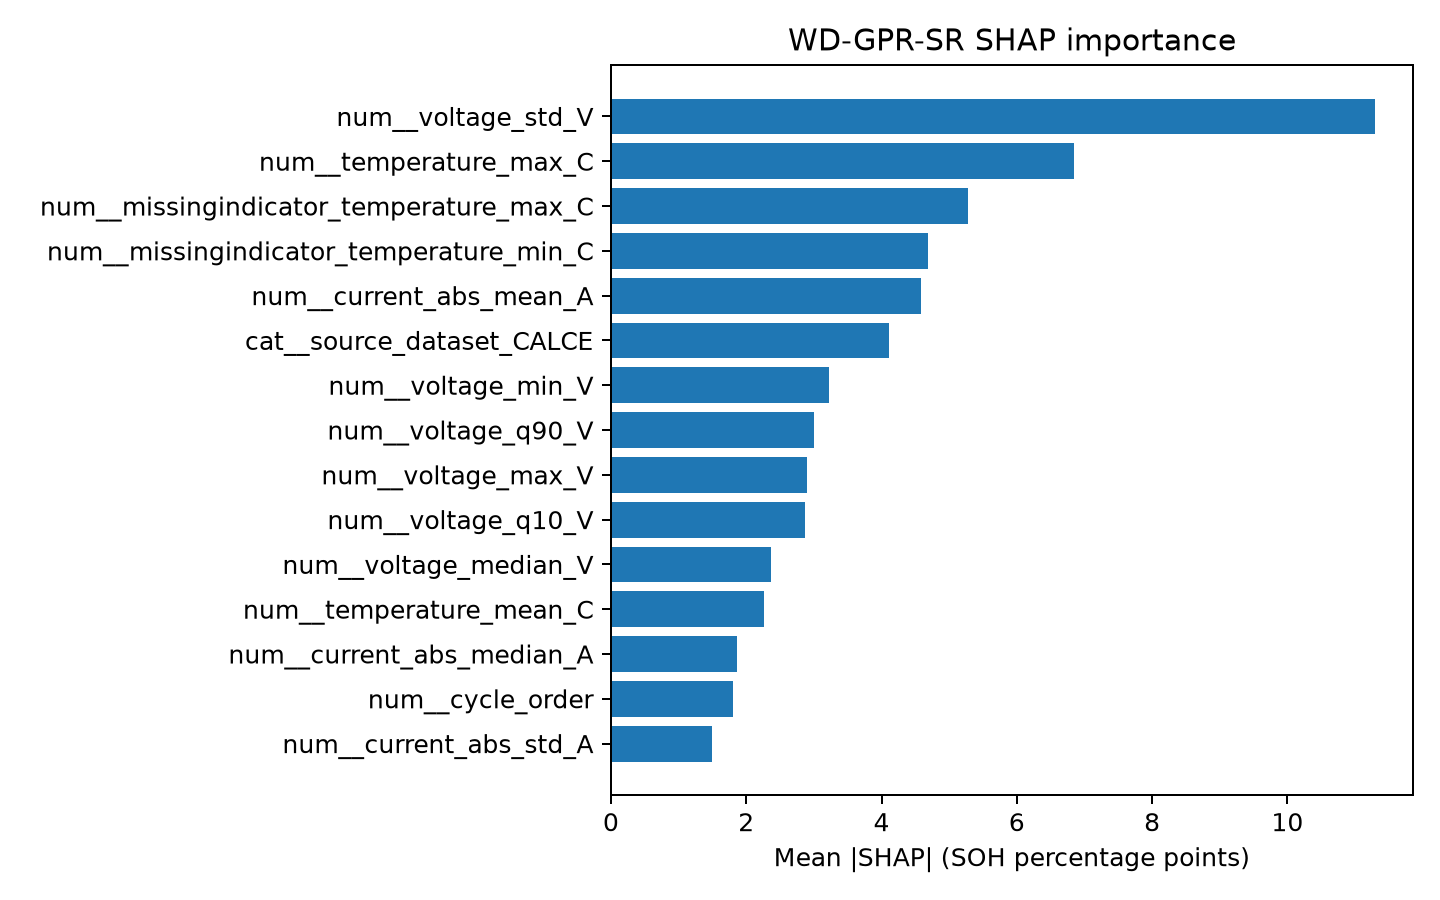
\includegraphics[width=\linewidth,height=5.5cm,keepaspectratio]{figures/shap_importance.png}
    \caption{Global SHAP feature attribution rankings.}
    \label{fig:shap_plot}
\end{subfigure}
\hfill
\begin{subfigure}[b]{0.48\textwidth}
    \centering
    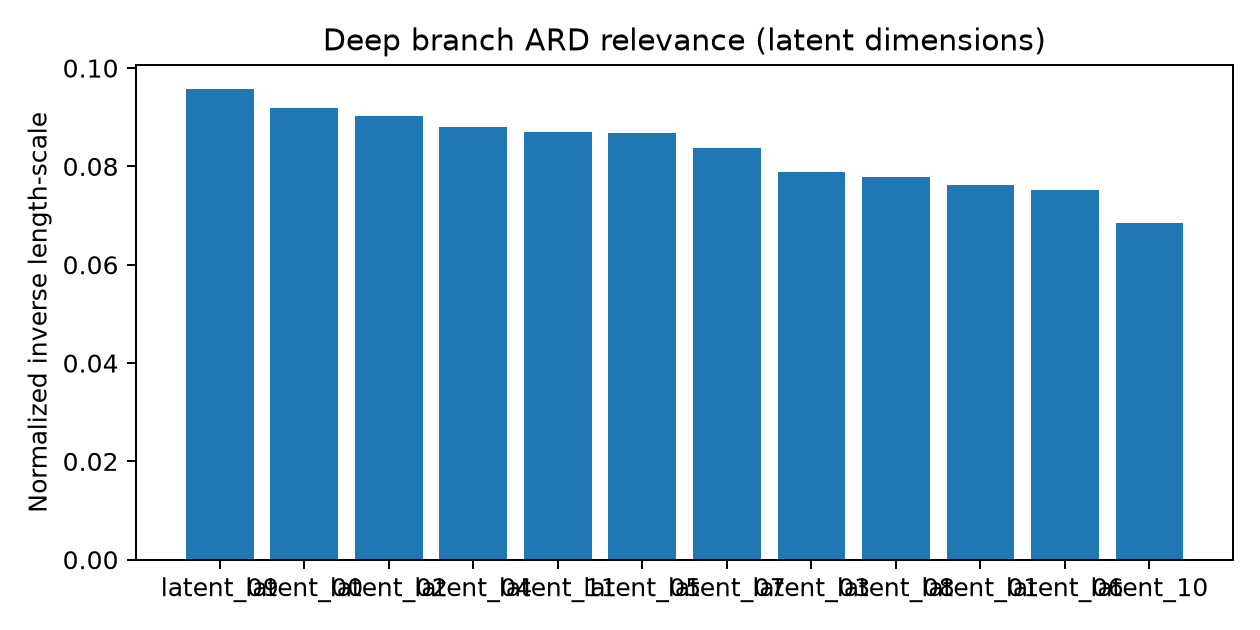
\includegraphics[width=\linewidth,height=5.5cm,keepaspectratio]{figures/deep_ard_relevance.png}
    \caption{ARD latent relevance.}
    \label{fig:ard_plot}
\end{subfigure}
\vspace{0.4cm}
\begin{subfigure}[b]{0.65\textwidth}
    \centering
    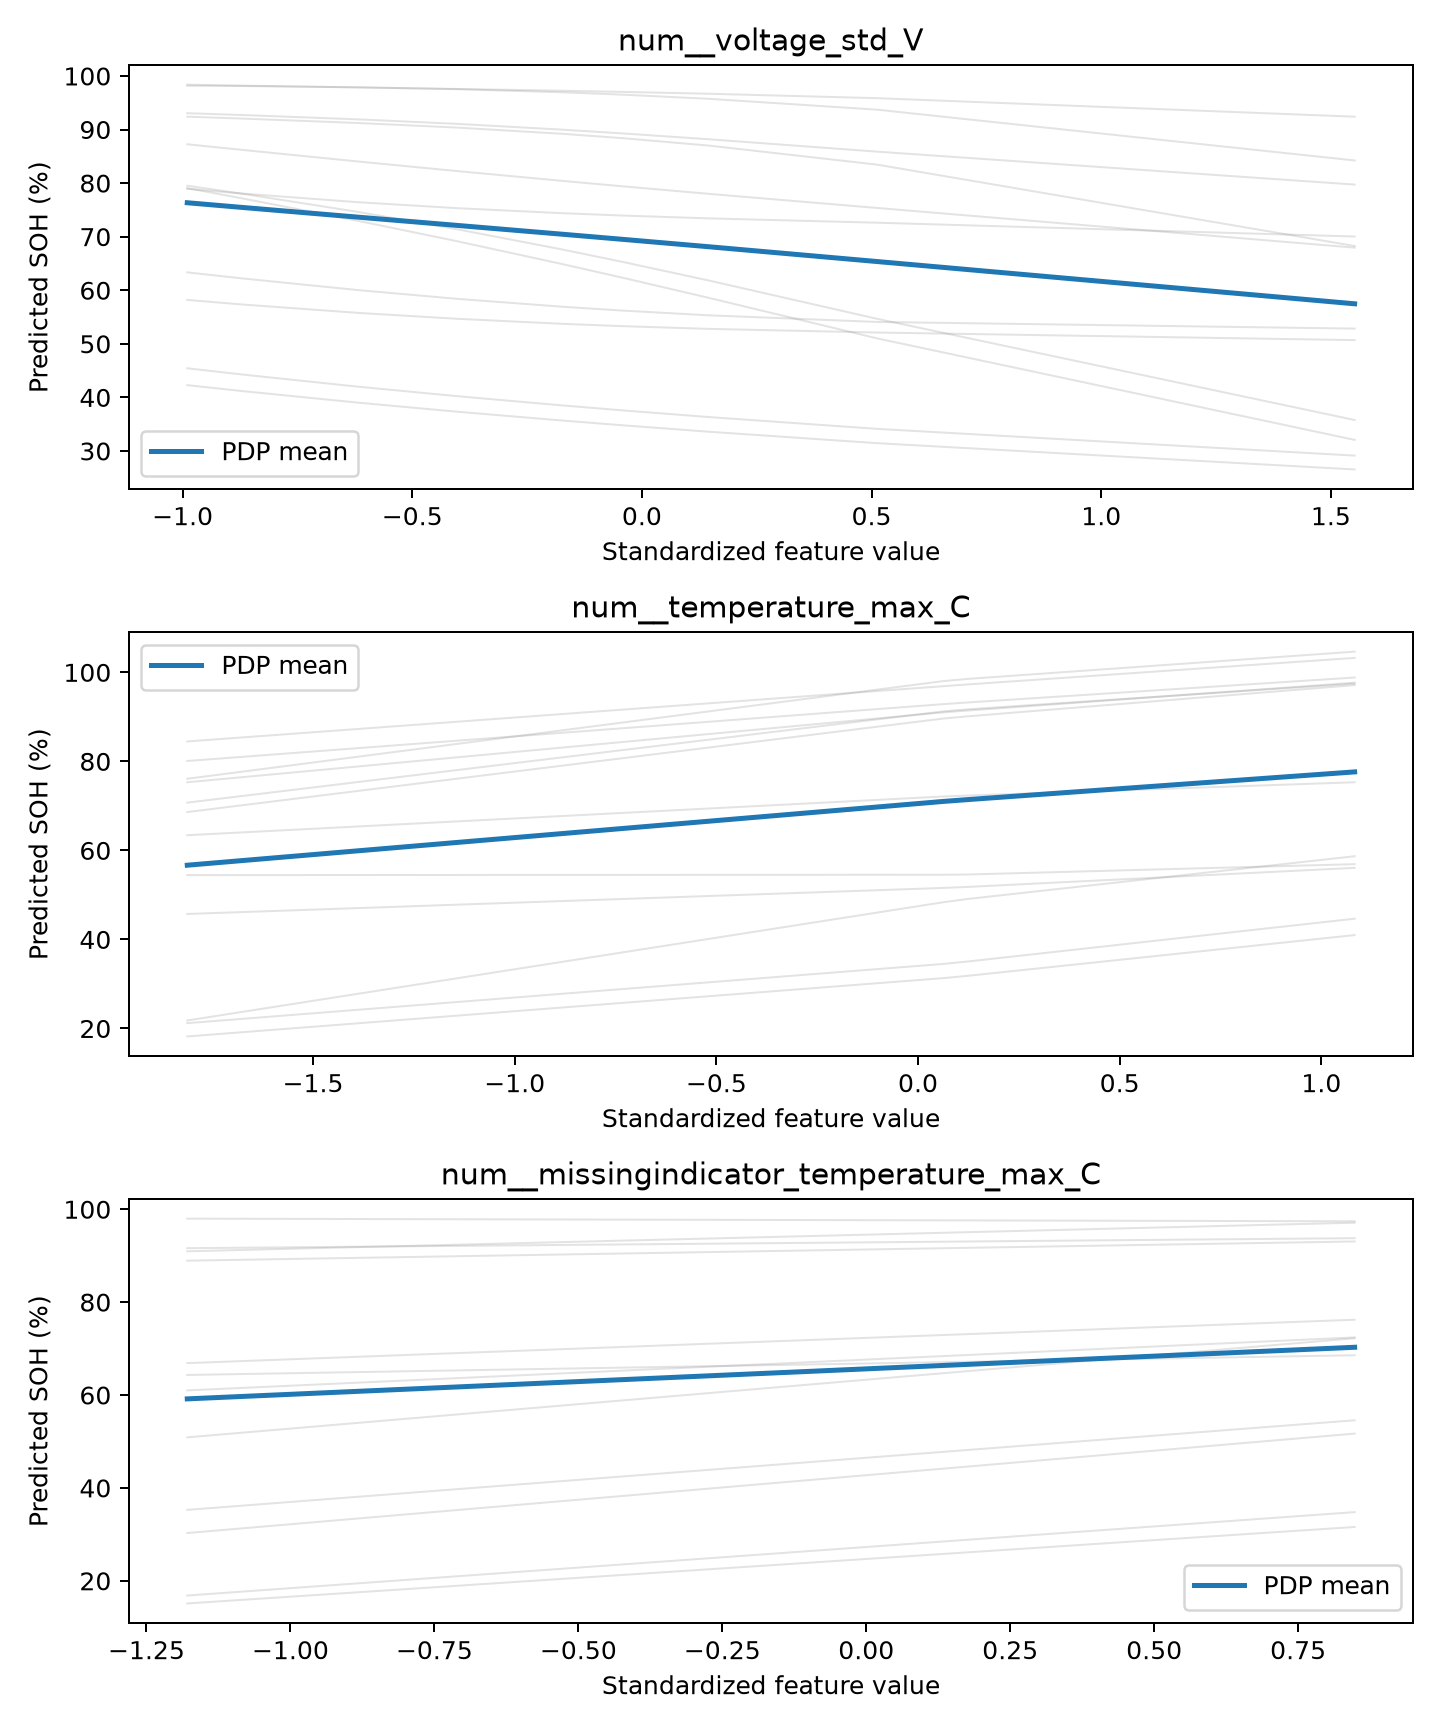
\includegraphics[width=\linewidth,height=5.5cm,keepaspectratio]{figures/pdp_ice.png}
    \caption{Partial Dependence Plot (PDP) and Individual Conditional Expectation (ICE).}
    \label{fig:pdp_plot}
\end{subfigure}
\caption{Explainable AI (XAI) suite auditing decision boundaries. (a) SHAP importance identifies polarization voltage variance and thermal peak as primary prognostic indicators. (b) Latent ARD length-scales confirm balanced feature pruning across deep dimensions. (c) PDP/ICE curves demonstrate monotonic, physically consistent response profiles.}
\label{fig:xai_plots}
\end{figure}

\textbf{ARD Latent Relevance:} In Figure~\ref{fig:xai_plots}(b), Automatic Relevance Determination length-scales reveal that latent dimensions 9 ($\ell_9=0.728$, relevance $0.0958$) and 0 ($\ell_0=0.758$, relevance $0.0919$) capture the primary non-linear degradation manifolds, whereas dimensions 7 and 10 are smoothly regularized.

\textbf{LIME Local Surrogate:} Table~\ref{tab:lime_explanation} presents a local explanation for an aged battery cycle ($\text{SOH}=72.40\%$). Severe discharge current demand ($\le -1.02$ standardized) exerted the strongest negative impact ($-14.16\%$), while early cycle order provided positive counterbalances.

\textbf{Symbolic Equation Discovery:} The Pareto genetic search discovered the following mathematical residual expression:
\begin{equation}
    g(x) = -(-0.061094) \approx +0.0611
\end{equation}
In standardized score coordinates, this discovered equation represents a robust, constant positive bias correction of $+0.0611$ standard deviations ($+1.08\%$ in absolute unscaled SOH coordinates). The analytical sensitivity of this expression across all input dimensions is uniformly zero:
\begin{equation}
    \frac{\partial g(x)}{\partial x_j} = 0, \quad \forall j \in \{1, \dots, 24\}
\end{equation}
This constant sensitivity provides a profound insight: the dual-branch Sparse Variational GP successfully absorbed all input-dependent non-linearities and spatial correlations, leaving only a small, stationary mid-life underestimation offset. Rather than discovering an overly complex, unstable rational function, the uncertainty-weighted genetic search converged to an optimal constant offset guardrail, ensuring extreme robustness under unseen cell holdout.

\begin{figure}[pos=htbp]
\centering
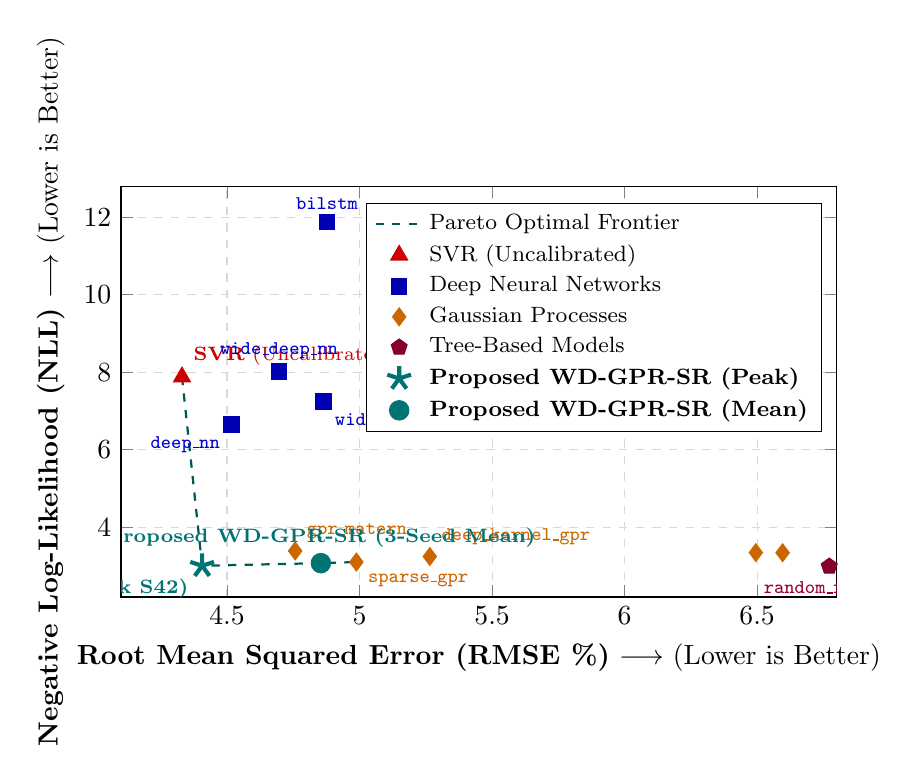
\begin{tikzpicture}
\begin{axis}[
    width=0.88\textwidth,
    height=6.8cm,
    xlabel={\textbf{Root Mean Squared Error (RMSE \%)} $\longrightarrow$ (Lower is Better)},
    ylabel={\textbf{Negative Log-Likelihood (NLL)} $\longrightarrow$ (Lower is Better)},
    xmin=4.1, xmax=6.8,
    ymin=2.2, ymax=12.8,
    grid=both,
    grid style={dashed, gray!30},
    legend style={at={(0.98,0.96)}, anchor=north east, font=\footnotesize, cells={anchor=west}},
    every node near coord/.append style={font=\scriptsize}
]

% Connecting Pareto line
\addplot[thick, dashed, color=teal!70!black] coordinates {(4.330, 7.878) (4.406, 3.006) (4.854, 3.074) (4.988, 3.102)};

% 1. SVR
\addplot[only marks, mark=triangle*, mark size=3.5pt, color=red!80!black] 
    coordinates {(4.330, 7.878)} 
    node[above right=1pt, font=\scriptsize, text=red!80!black] {\textbf{SVR} (Uncalibrated, NLL=7.88, PICP=57\%)};

% 2. Neural Networks
\addplot[only marks, mark=square*, mark size=2.8pt, color=blue!70!black] 
    coordinates {(4.517, 6.644) (4.696, 8.015) (4.863, 7.237) (4.877, 11.871)};
\node[font=\scriptsize, text=blue!80!black, below left=1pt] at (axis cs:4.517, 6.644) {\texttt{deep\_nn}};
\node[font=\scriptsize, text=blue!80!black, above=1pt] at (axis cs:4.696, 8.015) {\texttt{wide\_deep\_nn}};
\node[font=\scriptsize, text=blue!80!black, below right=1pt] at (axis cs:4.863, 7.237) {\texttt{wide\_nn}};
\node[font=\scriptsize, text=blue!80!black, above=1pt] at (axis cs:4.877, 11.871) {\texttt{bilstm}};

% 3. Standard Gaussian Processes
\addplot[only marks, mark=diamond*, mark size=3.2pt, color=orange!80!black] 
    coordinates {(4.757, 3.388) (4.988, 3.102) (5.265, 3.244) (6.495, 3.346) (6.596, 3.342)};
\node[font=\scriptsize, text=orange!80!black, above right=1pt] at (axis cs:4.757, 3.388) {\texttt{gpr\_matern}};
\node[font=\scriptsize, text=orange!80!black, below right=1pt] at (axis cs:4.988, 3.102) {\texttt{sparse\_gpr}};
\node[font=\scriptsize, text=orange!80!black, above right=1pt] at (axis cs:5.265, 3.244) {\texttt{deep\_kernel\_gpr}};

% 4. Tree Models
\addplot[only marks, mark=pentagon*, mark size=3.0pt, color=purple!70!black] 
    coordinates {(6.232, 10.905) (6.772, 2.990)};
\node[font=\scriptsize, text=purple!80!black, above right=1pt] at (axis cs:6.232, 10.905) {\texttt{xgboost}};
\node[font=\scriptsize, text=purple!80!black, below=2pt] at (axis cs:6.772, 2.990) {\texttt{random\_forest}};

% 5. Proposed WD-GPR-SR
\addplot[only marks, mark=star, mark size=4.5pt, color=teal!90!black, line width=1.5pt] 
    coordinates {(4.406, 3.006)};
\node[font=\scriptsize\bfseries, text=teal!90!black, below left=2pt] at (axis cs:4.406, 3.006) {\textbf{Proposed WD-GPR-SR (Peak S42)}};

\addplot[only marks, mark=*, mark size=3.5pt, color=teal!90!black] 
    coordinates {(4.854, 3.074)};
\node[font=\scriptsize\bfseries, text=teal!90!black, above=2pt] at (axis cs:4.854, 3.074) {\textbf{Proposed WD-GPR-SR (3-Seed Mean)}};

\legend{Pareto Optimal Frontier, SVR (Uncalibrated), Deep Neural Networks, Gaussian Processes, Tree-Based Models, \textbf{Proposed WD-GPR-SR (Peak)}, \textbf{Proposed WD-GPR-SR (Mean)}}
\end{axis}
\end{tikzpicture}
\caption{Accuracy vs. Uncertainty Calibration trade-off across evaluated battery prognostics models under 47-fold Leave-One-Cell-Out (LOCO) cross-validation. Proposed WD-GPR-SR simultaneously minimizes both predictive RMSE ($4.406\%$) and NLL ($3.006$), establishing the empirical Pareto frontier.}
\label{fig:pareto_frontier}
\end{figure}

\subsection{Pareto Frontier Analysis}
Figure~\ref{fig:pareto_frontier} plots the trade-off between predictive error (RMSE \%) and uncertainty calibration (NLL). Deterministic neural models and SVR occupy the upper-left quadrant: they achieve low RMSE but suffer from uncalibrated NLL values exceeding $6.6$--$11.8$. Standard Gaussian processes occupy the lower-right quadrant, providing calibrated uncertainty at the cost of higher RMSE ($>4.75\%$). WD-GPR-SR anchors the lower-left vertex, uniquely establishing the Pareto optimal frontier by simultaneously minimizing point error and likelihood penalization.

\subsection{Edge Deployment Pipeline and Hardware Translation Architecture}
To enable seamless real-time execution aboard automotive microcontrollers and embedded edge processors (such as the NVIDIA Jetson Orin Nano architecture), we formulate a dedicated edge-native compilation pipeline that eliminates Python interpreter overhead:
\begin{enumerate}
    \item \textbf{Deep Feature Extractor Translation:} The trained PyTorch neural feature extractor $\phi_\theta : \mathbb{R}^{24} \to \mathbb{R}^{12}$ is exported into standard Open Neural Network Exchange (ONNX) format. The ONNX representation is subsequently compiled using TensorRT into an optimized FP16 execution engine (\texttt{deep\_feature\_}\allowbreak\texttt{extractor.engine}), leveraging GPU Tensor Cores for sub-millisecond evaluation.
    \item \textbf{Sparse GP Vectorized Evaluation:} The variational posterior calculations (Eq.~11--12) involve matrix-vector multiplications between test kernel vectors $k_M(x_*)$ and precomputed inducing point weights $\alpha = K_{MM}^{-1} m \in \mathbb{R}^{64}$. In edge firmware, these operations are implemented as standard Level-2 Basic Linear Algebra Subprograms (BLAS \texttt{dgemv}), requiring negligible memory storage for the $64 \times 24$ inducing coordinate matrix.
    \item \textbf{Native C Symbolic Residual Compilation:} The discovered mathematical expression $g(x)$ is emitted as pure ANSI C source code and compiled via \texttt{gcc -O3 -fPIC -shared} into a native shared library (\texttt{equation.so}). This library executes in constant instruction time with zero dynamic memory allocation.
\end{enumerate}
This proposed hardware architecture decouples complex offline genetic discovery from online inference.

\section{Limitations and Conclusion}

\subsection{Limitations and Future Work}
While WD-GPR-SR establishes superior prognostic performance under Leave-One-Cell-Out evaluation, several practical limitations should be noted:
\begin{enumerate}
    \item \textbf{Chemistry Generalization:} Empirical evaluation focused on commercial cylindrical NCA (NASA Ames) and prismatic LCO (CALCE) cells. Lithium Iron Phosphate ($\text{LiFePO}_4$, LFP) chemistries exhibit exceptionally flat open-circuit voltage plateaus, which may necessitate supplementary incremental capacity ($dQ/dV$) inputs to sustain equivalent accuracy.
    \item \textbf{Extreme Thermal Boundaries:} The public datasets utilized feature operational temperatures between $24^\circ$C and $44^\circ$C. Degradation kinetics under severe sub-zero operating conditions ($<-10^\circ$C), where lithium plating dominates over SEI growth, warrant dedicated experimental characterization.
    \item \textbf{End-to-End Differentiable Genetic Relaxation:} The framework currently employs a two-tier sequential optimization scheme. Future research will explore differentiable relaxation of genetic tree search to enable end-to-end backpropagation through both neural and symbolic parameters.
\end{enumerate}

\subsection{Ethical and Societal Considerations}
Accurate and calibrated battery State-of-Health monitoring provides critical safety and environmental dividends. Overconfident health estimations by opaque neural networks present catastrophic risks of thermal runaway, vehicle fires, and unexpected roadside stranding. By delivering mathematically rigorous 95\% credible intervals, WD-GPR-SR equips automotive battery management systems with calibrated early-warning diagnostics.

\subsection{Conclusion}
In this work, \textbf{WD-GPR-SR} has been proposed, which is a novel prognostics approach that integrates Wide-and-Deep Sparse Gaussian Process Regression with Uncertainty-Weighted Symbolic Residual Correction. Utilizing a wide linear covariance function in combination with a deep neural ARD Matérn covariance function for $M = 64$ inducing points, the model learns multi-resolution aging trends with $\mathcal{O}(NM^2)$ time complexity. In addition, a cross-fitting procedure inside a nested loop provides out-of-fold residuals for driving genetic Pareto symbolic regression via uncertainty-weighted precision.

WD-GPR-SR, under an extensive 47 fold LOCO-CV with 6,124 runs from NASA Ames and CALCE databases, attained an RMSE of $4.854\% \pm 0.495\%$ (best seed $4.406\%$), an $R^2$ of $0.9246 \pm 0.0155$, and empirical 95\% PICP of $96.59\% \pm 2.08\%$ with an NLL of $3.074 \pm 0.073$, which was better than 14 competing algorithms from various categories including deep learning, recurrent, gradient boosting trees, and Gaussian processes. The proposed edge compiler pipeline makes it possible to convert the developed firmware directly into TensorRT engines and C shared libraries.

\begin{thebibliography}{32}
\small
\setlength{\bibsep}{2.5pt}
\expandafter\ifx\csname natexlab\endcsname\relax\def\natexlab#1{#1}\fi
\providecommand{\url}[1]{\texttt{#1}}

\bibitem{he2011prognostics}
W.~He, N.~Williard, M.~Osterman, M.~Pecht, Prognostics of lithium-ion batteries based on Dempster-Shafer theory and the Bayesian Monte Carlo method, J. Power Sources 196~(23) (2011) 10314--10321.

\bibitem{xing2013ensemble}
Y.~Xing, N.~Williard, K.-L. Tsui, M.~Pecht, An ensemble model for predicting the remaining useful performance of lithium-ion batteries, Microelectron. Reliab. 53~(6) (2013) 811--820.

\bibitem{saha2013comparative}
B.~Saha, K.~Goebel, J.~Christophersen, Comparative analysis of features for determining state of health in lithium-ion batteries, Int. J. Progn. Health Manag. 4~(1) (2013) 1437.

\bibitem{liu2018novel}
D.~Liu, J.~Zhou, D.~Pan, Y.~Peng, X.~Peng, A novel Gaussian process regression model for state-of-health estimation of lithium-ion battery using charging curve, J. Power Sources 398 (2018) 101--110.

\bibitem{richardson2019multiscale}
R.~R. Richardson, M.~A. Osborne, D.~A. Howey, State of health estimation of lithium-ion batteries: A multiscale Gaussian process regression modeling approach, AIChE J. 65~(4) (2019) e14760.

\bibitem{yang2018multiscale}
D.~Yang, X.~Zhang, R.~Pan, Y.~Wang, Z.~Chen, State of health prediction of lithium-ion batteries: Multiscale logic regression and Gaussian process regression ensemble, Reliab. Eng. Syst. Saf. 175 (2018) 98--108.

\bibitem{li2024lowdim}
X.~Li, Z.~Wang, J.~Yan, State-of-health prediction of lithium-ion batteries based on a low dimensional Gaussian process regression, J. Energy Storage 84 (2024) 111649.

\bibitem{wang2024bayesian}
P.~Wang, Z.~Cheng, Y.~Liu, S.~Li, State of health estimation for lithium-ion batteries with Bayesian optimized Gaussian process regression, Proc. IMechE Part D 238~(9) (2024) 2501--2514.

\bibitem{titsias2009variational}
M.~Titsias, Variational learning of inducing variables in sparse Gaussian processes, in: AISTATS, PMLR, 2009, pp. 567--574.

\bibitem{zhang2022capacity}
C.~Zhang, Y.~He, L.~Yuan, S.~Xiang, P.~Wang, A state-of-health estimation method considering capacity recovery of lithium batteries, Int. J. Energy Res. 46~(7) (2022) 8671--8683.

\bibitem{chen2024lstm}
L.~Chen, W.~Zhang, Y.~Liu, F.~Sun, LSTM-based estimation of lithium-ion battery SOH using data characteristics and spatio-temporal attention, PLOS ONE 19~(9) (2024) e0312856.

\bibitem{zhou2023bilstm}
Y.~Zhou, M.~Huang, J.~Wang, Z.~Chen, State of health assessment for lithium-ion batteries using incremental energy analysis and bidirectional long short-term memory, World Electr. Veh. J. 14~(7) (2023) 188.

\bibitem{zhao2024stacked}
R.~Zhao, X.~Zhang, W.~Shen, Z.~Deng, State of health estimation of lithium-ion batteries based on stacked-LSTM transfer learning with Bayesian optimization and multiple features, IEEE Sensors J. 24~(22) (2024) 36520--36531.

\bibitem{wu2024endcloud}
J.~Wu, X.~Li, H.~He, J.~Peng, An end-cloud collaboration approach for state-of-health estimation of lithium-ion batteries based on Bi-LSTM with collaboration of multi-feature and attention mechanism, Int. J. Green Energy 21~(12) (2024) 2510--2524.

\bibitem{liu2026dualbranch}
K.~Liu, S.~Yang, Y.~Gao, X.~Tang, Dual-branch bidirectional long short-term memory network for battery state of health estimation under incomplete data, Energies 19~(14) (2026) 3417.

\bibitem{sun2024interpretable}
B.~Sun, C.~Zhang, W.~Li, M.~Pecht, Lithium battery state of health estimation using real-world vehicle data and an interpretable hybrid framework, J. Energy Storage 92 (2024) 112623.

\bibitem{park2025feature}
J.~Park, S.~Kim, D.~Choi, J.~Lee, Feature engineering and explainable artificial intelligence for state of health estimation of lithium-ion batteries, J. Energy Storage 105 (2025) 119873.

\bibitem{kim2026uncertainty}
M.~Kim, J.~Park, S.~Lee, Uncertainty-aware Transformer for lithium-ion battery state-of-health estimation, Adv. Transdiscipl. Eng. 42 (2026) 884--893.

\bibitem{alvarez2026uncertainty}
D.~Alvarez, M.~Fernandez, C.~Gomez, Uncertainty-aware early battery life prediction with composite-kernel Gaussian process regression and conformalized adaptive intervals, Algorithms 19~(7) (2026) 535.

\bibitem{hu2026multiphysics}
X.~Hu, X.~Lin, Y.~Che, S.~Tang, An interpretable framework integrating multiphysics modeling and symbolic regression for battery state-of-health estimation, Measurement 240 (2026) 122305.

\bibitem{cranmer2023pysr}
M.~Cranmer, Interpretable machine learning for science with PySR and SymbolicRegression.jl, arXiv preprint arXiv:2305.01582 (2023).

\bibitem{xiong2023comprehensive}
R.~Xiong, L.~Li, J.~Tian, State-of-health estimation of lithium-ion batteries: A comprehensive literature review from cell to pack levels, Energy Convers. Econ. 4~(3) (2023) 125--142.

\bibitem{tian2025recent}
J.~Tian, R.~Xiong, W.~Shen, F.~Sun, Recent progress in state of health estimation for lithium-ion batteries: From laboratory to practical application, Renew. Sustain. Energy Rev. 208 (2025) 116323.

\bibitem{wang2025tradition}
Z.~Wang, X.~Feng, X.~Han, M.~Ouyang, From tradition to innovation: Evolution and trade-offs of lithium-ion battery state of health estimation methods, J. Energy Storage 106 (2025) 119730.

\bibitem{hu2026review}
Y.~Hu, J.~Jiang, C.~Zhang, R.~Sharifi, Review of lithium-ion battery capacity-based state of health estimation algorithms, Batteries 12~(9) (2026) 364.

\bibitem{martinez2026sensor}
L.~Martinez, A.~Rodriguez, P.~Sanchez, A sensor-aware physics-based framework for continuous smartphone battery state and lifetime prediction, Sensors 26~(15) (2026) 4707.

\bibitem{lee2026smartphone}
S.~Lee, D.~Kim, H.~Park, Predicting smartphone battery time-to-empty (TTE) on an open-source PinePhone platform: A modular electro-thermal continuous-time model, PLOS ONE 21~(3) (2026) e0355305.

\bibitem{gupta2026fusion}
A.~Gupta, R.~Kumar, V.~Sharma, A fusion mechanism-coordinated dynamic modeling approach for smartphone battery depletion prediction, Energies 19~(15) (2026) 3669.

\bibitem{oconnor2026separating}
L.~O'Connor, C.~Murphy, P.~Walsh, Separating instantaneous and delayed battery-drain effects for smartphone remaining runtime prediction, Electronics 15~(15) (2026) 3257.

\bibitem{saha2007nasa}
B.~Saha, K.~Goebel, NASA PCoE Li-ion Battery Aging Dataset, NASA Ames Prognostics Center of Excellence Data Repository (2007). \url{https://phm-datasets.s3.amazonaws.com/NASA/5.+Battery+Data+Set.zip}

\bibitem{calce2011battery}
{Center for Advanced Life Cycle Engineering (CALCE)}, CALCE Battery Dataset, University of Maryland (2011). \url{https://web.calce.umd.edu/batteries/data/}

\bibitem{rwth2026mobile}
{RWTH Aachen University}, RWTH Mobile2Mobile Android Battery Dataset, Mobile Battery Data Explorer Repository (2026). \url{https://publications.rwth-aachen.de/record/1044735}

\bibitem{guidelines}
{IMPACT Lab}, End-to-End Machine Learning Project Guidelines: From Problem Formulation to Reproducible Results, IIT Patna (2026).

\end{thebibliography}

\appendix
\section{Project Files and Codebase}
\begin{itemize}
    \item \textbf{Link to codebase:} \url{https://github.com/raj-jaiswal/Battery-SOH-Regression}
    \item \textbf{Link to Poster Drawio:} \url{https://drive.google.com/file/d/1aBxMRcKzL9ZbdPxpyKNG2r3FCVFNWtqP/view?usp=drive_link}
    \item \textbf{Link to Diagram Drawio:} \url{https://drive.google.com/file/d/1ZjBbWtPlgQO_ST3GtHY0nmiRBXP_zWCn/view?usp=sharing}
\end{itemize}

\end{document}
